\documentclass[a4paper]{IEEEtran}
\usepackage[utf8]{inputenc}
%\usepackage{epstopdf}
%\usepackage[spanish]{babel}
\usepackage[cmex10]{amsmath}
\interdisplaylinepenalty=2500
\usepackage{amsfonts}
\usepackage{amssymb}
\usepackage{graphicx}
\usepackage{verbatim}
\usepackage{array}
\usepackage{multirow}
\usepackage{dcolumn}
\usepackage{color}
\usepackage[noadjust]{cite}
\usepackage{url}
\usepackage{balance}
\usepackage[usenames,dvipsnames]{xcolor}
\usepackage{algorithm}
\usepackage[noend]{algpseudocode}
\DeclareGraphicsExtensions{.eps}

\makeatletter
\def\BState{\State\hskip-\ALG@thistlm}
\makeatother


\DeclareMathOperator*{\Max}{max}
\DeclareMathOperator*{\Min}{min}
\DeclareMathOperator*{\argmin}{arg\,min}
\DeclareMathOperator*{\Maximize}{Maximize}

\begin{document}
\title{Generating joint scenarios of renewable energy sources: the case for non-Gaussian models with time varying parameters}

\author{Henrique Hoeltgebaum,
	Cristiano Fernandes, and
	Alexandre Street, \IEEEmembership{Senior Member IEEE}
	
	
	\thanks{This work was partially supported by the R\&D project ANEEL PD-7625-0001/2013.}
	\thanks{Henrique Hoeltgebaum, Cristiano Fernandes and Alexandre Street are with the Electrical Engineering Department, Pontifical Catholic University of Rio de Janeiro (PUC-Rio), Rio de Janeiro, RJ, Brazil (e-mail: \mbox{hhhelfer@ele.puc-rio.br}; \mbox{cris@ele.puc-rio.br}; \mbox{street@ele.puc-rio.br}).}
}


\maketitle
\begin{abstract}
	The development of medium- and long-term studies for power-system operation and planning under uncertainty of renewable generation is one of the key challenges faced by planners and market players in most of the power system worldwide. There is a vast literature on stochastic optimization models devoted to address the relevant issues on power system operation and planning applications. Notwithstanding, few papers focus on addressing the gaps on the subject of joint scenario generation despite the high sensibility of the stochastic optimization models with regard to their input scenarios. The characterization wind power generation (WPG) stochastic processes to devise time- and spatial-dependent scenarios, based on simulation procedures, for one to few years horizon is a difficult task. Multiple regimes and non Gaussian distributions are one of the main issues faced in both centralized and private planning/investment studies. In this paper a new methodology to simulate long-term joint scenarios for multivariate WPG time series is presented. The proposed framework is derived based on a new class of time-series model with time-varying parameters and arbitrary non Gaussian distribution, known as Generalized Auto Regressive Score models (GAS). GAS models provide a relevant flexibility and control of the simulated scenarios in long-run chronological Monte Carlo simulation procedures. In this work, we study the case of a beta PDF and spacial dependence is captured by an elliptical copula with time-varying correlation matrix. Case studies based on the Brazilian power system show that the proposed methodology is capable to address relevant issues that arise in long-term simulation studies. 
	
\end{abstract}

\begin{IEEEkeywords}
	Score driven models, wind power, probabilistic forecasting, time varying parameters, dynamic copula.
\end{IEEEkeywords}

% ========== ========== ========== ========== ========== 
% ===== Sec. I - Introduction ===== %
% ========== ========== ========== ========== ========== 

\section{Introduction}
\label{Introduction}

\IEEEPARstart{R}{enewable} energy expansion has been growing worldwide, mainly in response to governmental incentive for reducing greenhouse gas emissions. In particular, wind-power generation (WPG) is one of the largest sources of renewable energy, and according to the International Energy Agency, will respond to 18\% of global power by 2050  \cite{IntEnerAgency}. However the uncertainty associated with its non dispatchable nature may jeopardize reliability of electricity supply. In attempting to minimize this kind of risk it is highly desirable to produce reliable forecasts and scenarios for WPG time series. The importance of such scenarios emerges in many instance, as for example: (i) energy trading, (ii) unit commitment, (iii) grid expansion planning, and (iv) investment decisions (see (\cite{moreiraStreet,jabr2013robust,zhaoguan,Aderson2017}) and references therein). %Nevertheless, even though there is plenty of literature 
There is a vast literature on stochastic optimization models devoted to address the relevant issues on the aforementioned power system applications. Notwithstanding, few papers focus on addressing the gaps on the subject of joint scenario generation despite the high sensibility of the stochastic optimization models with regard to their input scenarios.


%In this paper, a methodology to generate long-term joint scenarios for time series of capacity factors (CF) associated with different wind plants is proposed. Modelling and simulating such a set of time series imposes two major challenges, namely: (i) the intrinsic non Gaussian nature of CF time series. (ii) the possibility of non linear dependence among these series. In order to properly address these two characteristics of CF time series we propose the use of a new class of time series models, the Generalized Autoregressive Score (GAS)  \cite{creal2013generalized} or Dynamic Conditional Score (DCS), following \cite{harvey2013dynamic}.%Another  strong seasonal pattern, which conventional autoregressive models cannot handle straightforward. To empirically illustrate such facts, we provide in Figure \ref{BoxPlots_IC_mensal} an annual plot of CF from one wind plant located at the Northeast of Brazil, namely Icaraizinho (here and after denoted as IC).

%\begin{figure}[htbp]
%\centering
%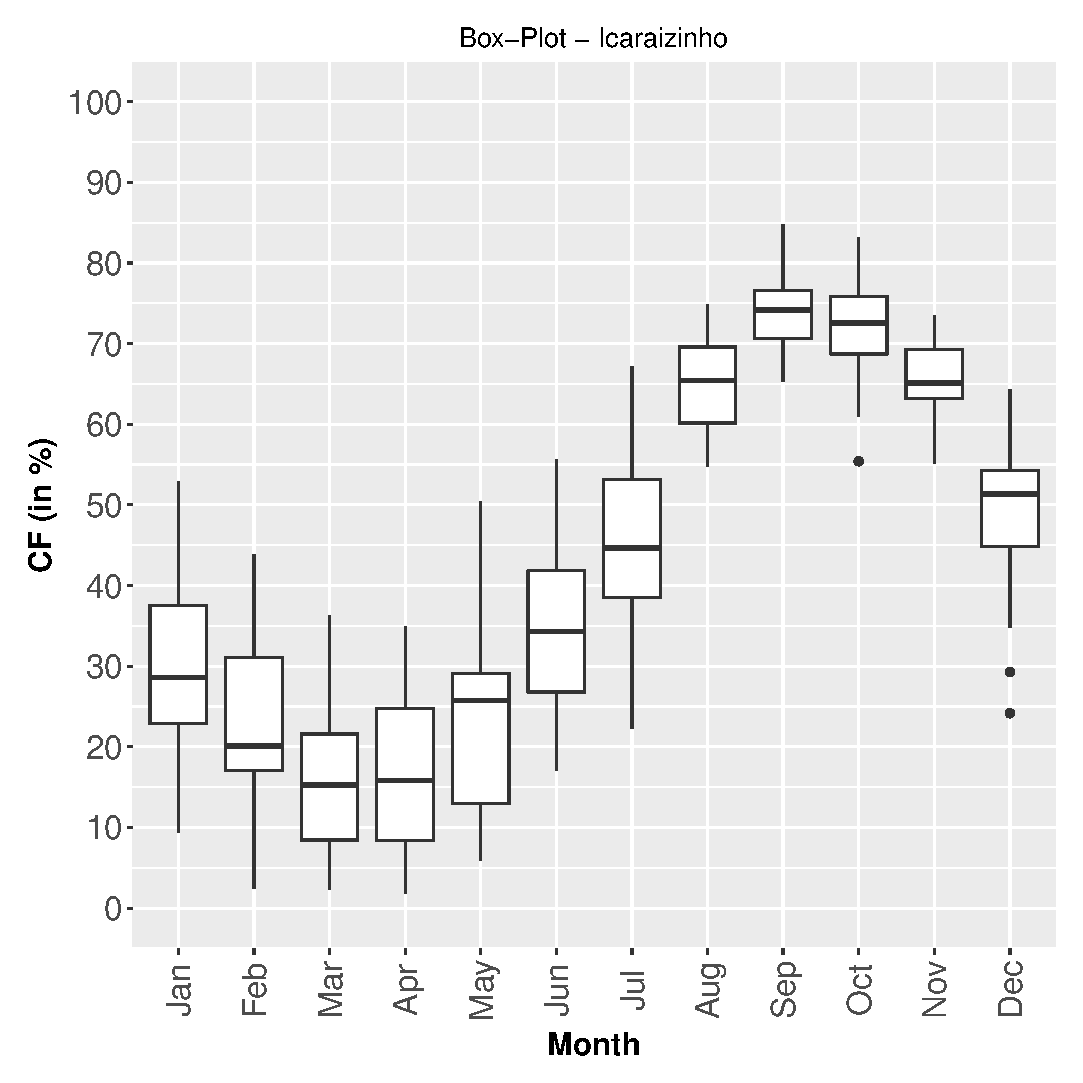
\includegraphics[height=7cm,width=7cm]{figures/BOXPLOT_IC.eps}
%\caption{Monthly capacity factor from a wind plant located at the Northest of Brazil. The time series ranges from January 1981 to December 2011.}
%\label{BoxPlots_IC_mensal}
%\end{figure}

%\begin{figure}[htbp]
%\centering
%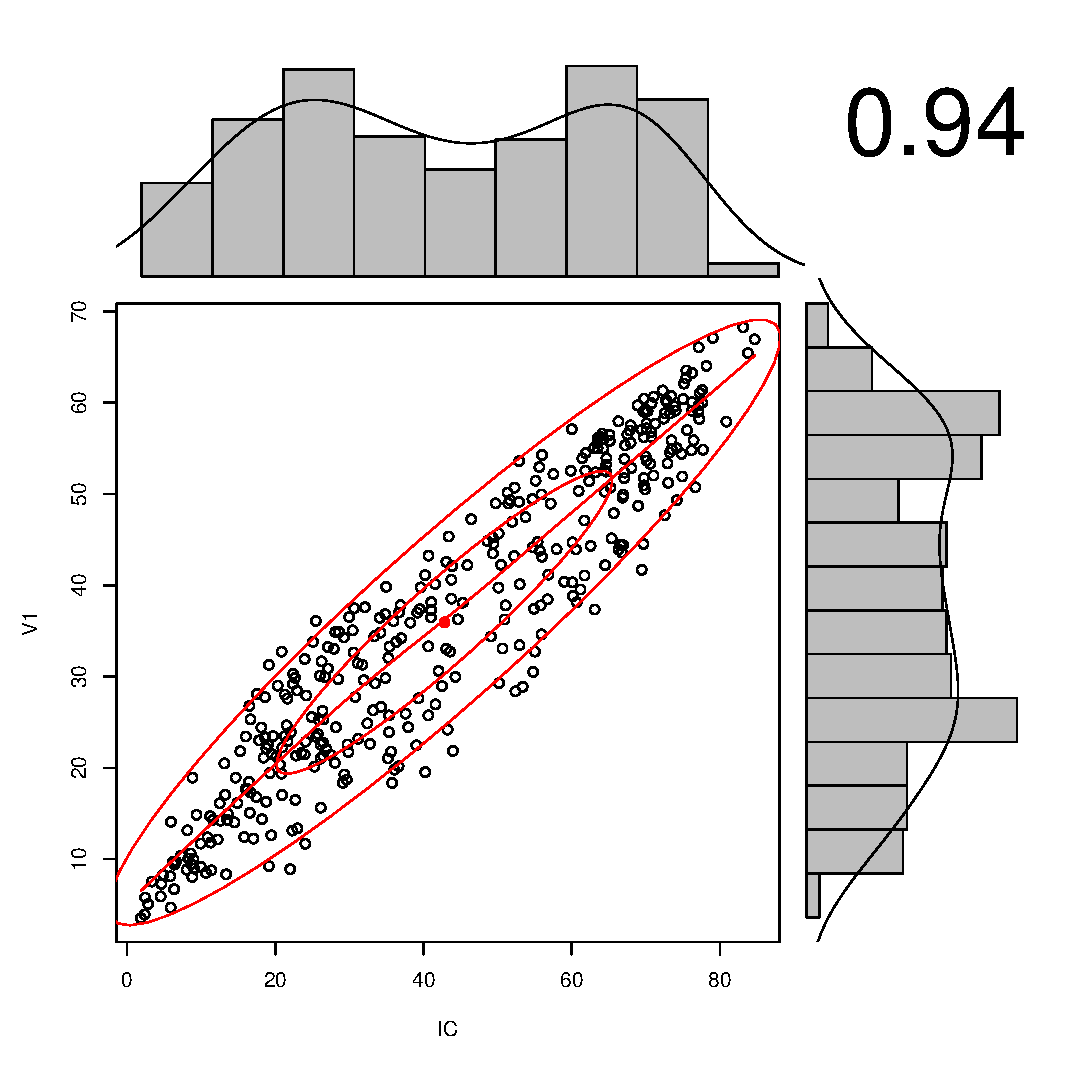
\includegraphics[height=5cm,width=6cm]{figures/HIST_ENxIC.eps}
%\caption{Scatterplot+Histogram ENxIC}
%\label{BoxPlots}
%\end{figure}
%
%\begin{figure}[htbp]
%\centering
%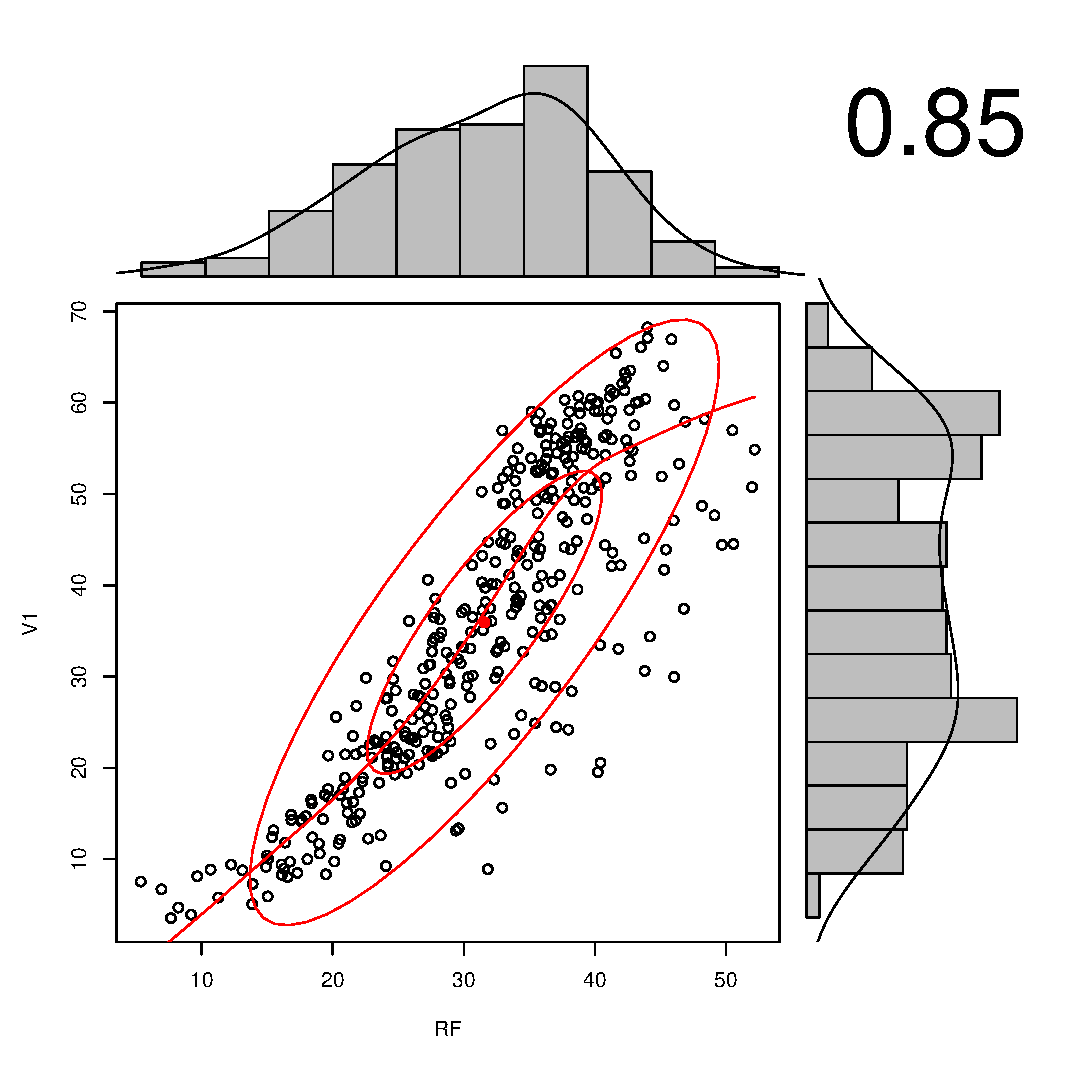
\includegraphics[height=5cm,width=6cm]{figures/HIST_RFxEN.eps}
%\caption{Scatterplot+Histogram RFxEN}
%\label{BoxPlots}
%\end{figure}
%
%\begin{figure}[htbp]
%\centering
%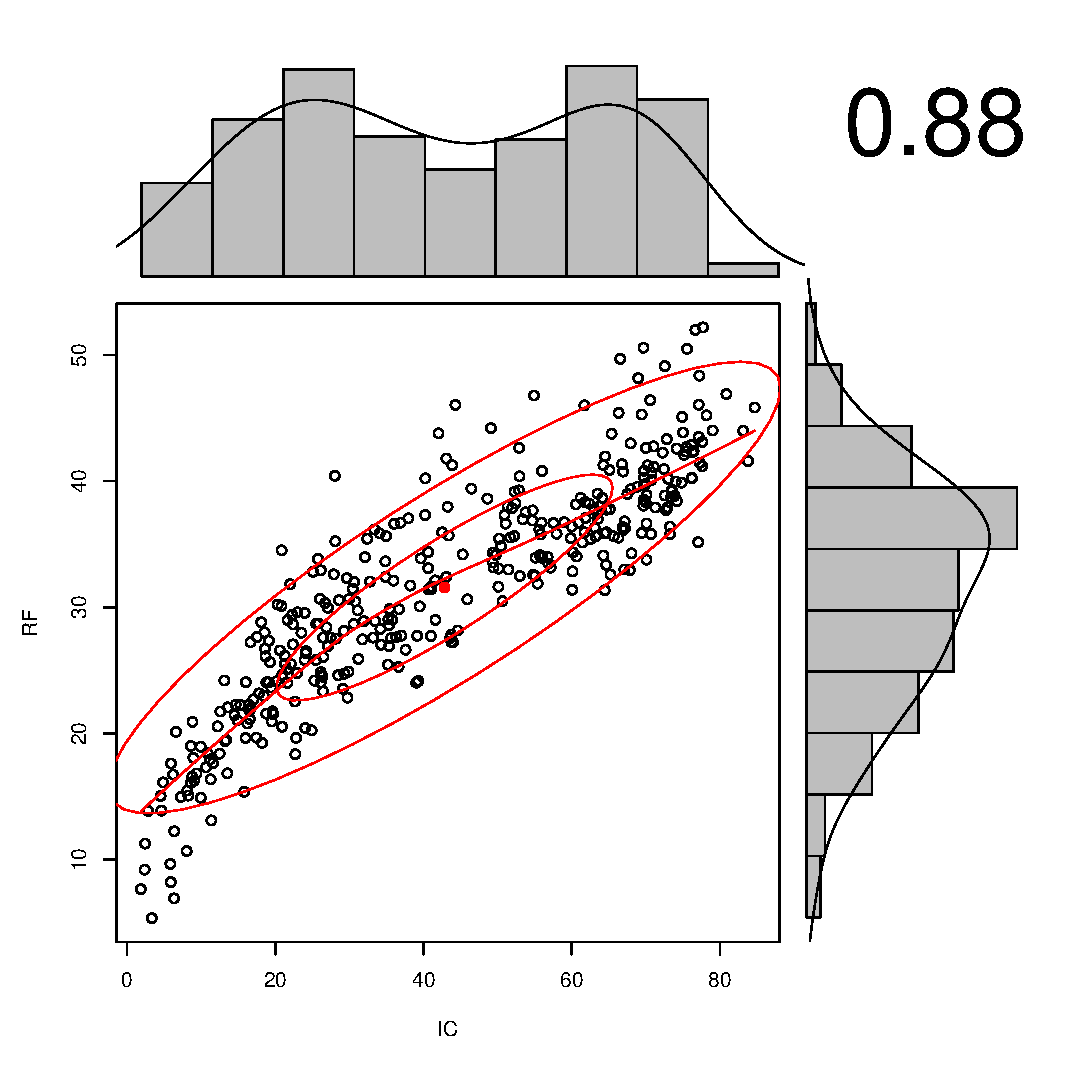
\includegraphics[height=5cm,width=6cm]{figures/HIST_RFxIC.eps}
%\caption{Scatterplot+Histogram RFxIC}
%\label{BoxPlots}
%\end{figure}
%
%
%
%\begin{figure}[htbp]
%\centering
%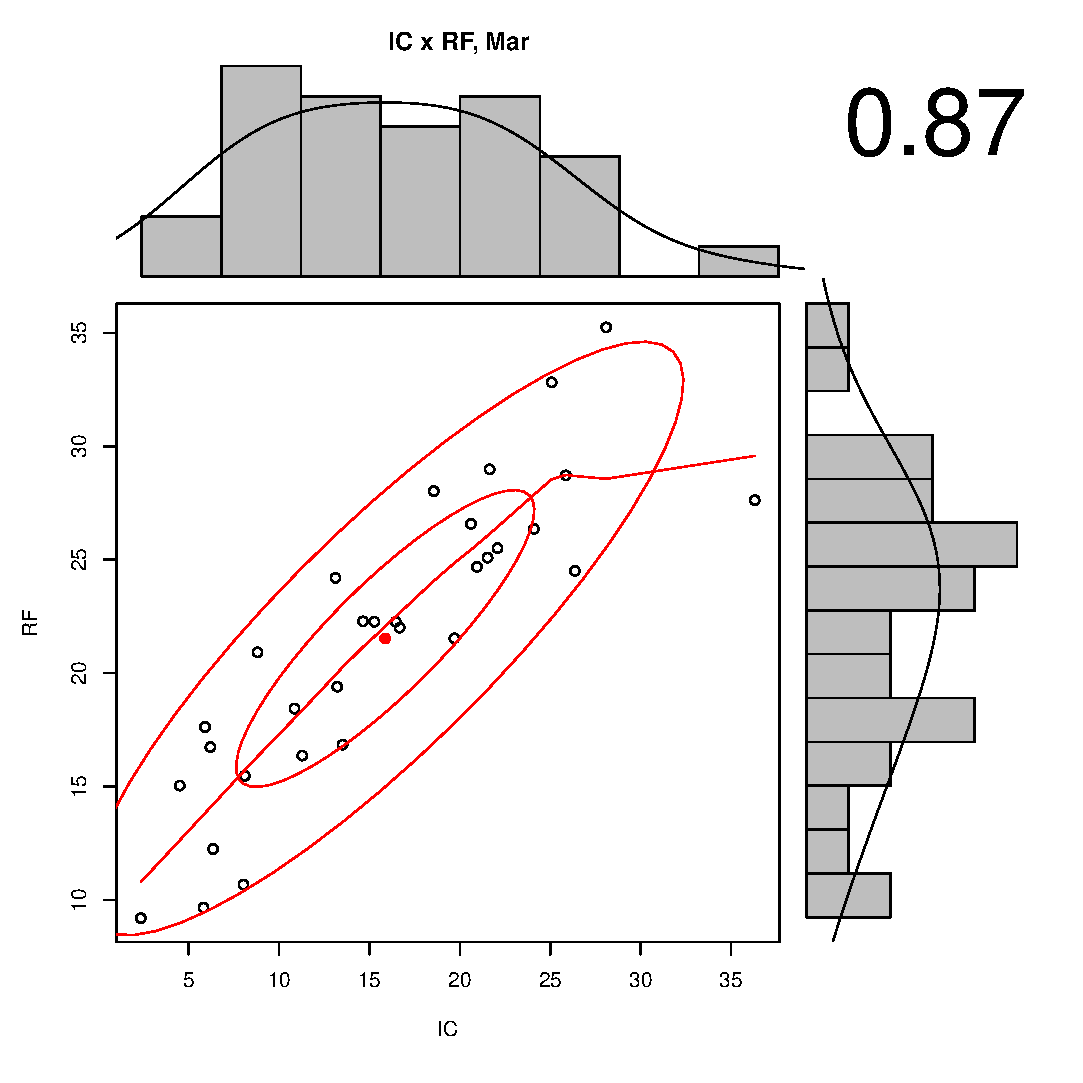
\includegraphics[height=2cm,width=2cm]{figures/HIST_ICxRF_mesMar.eps}
%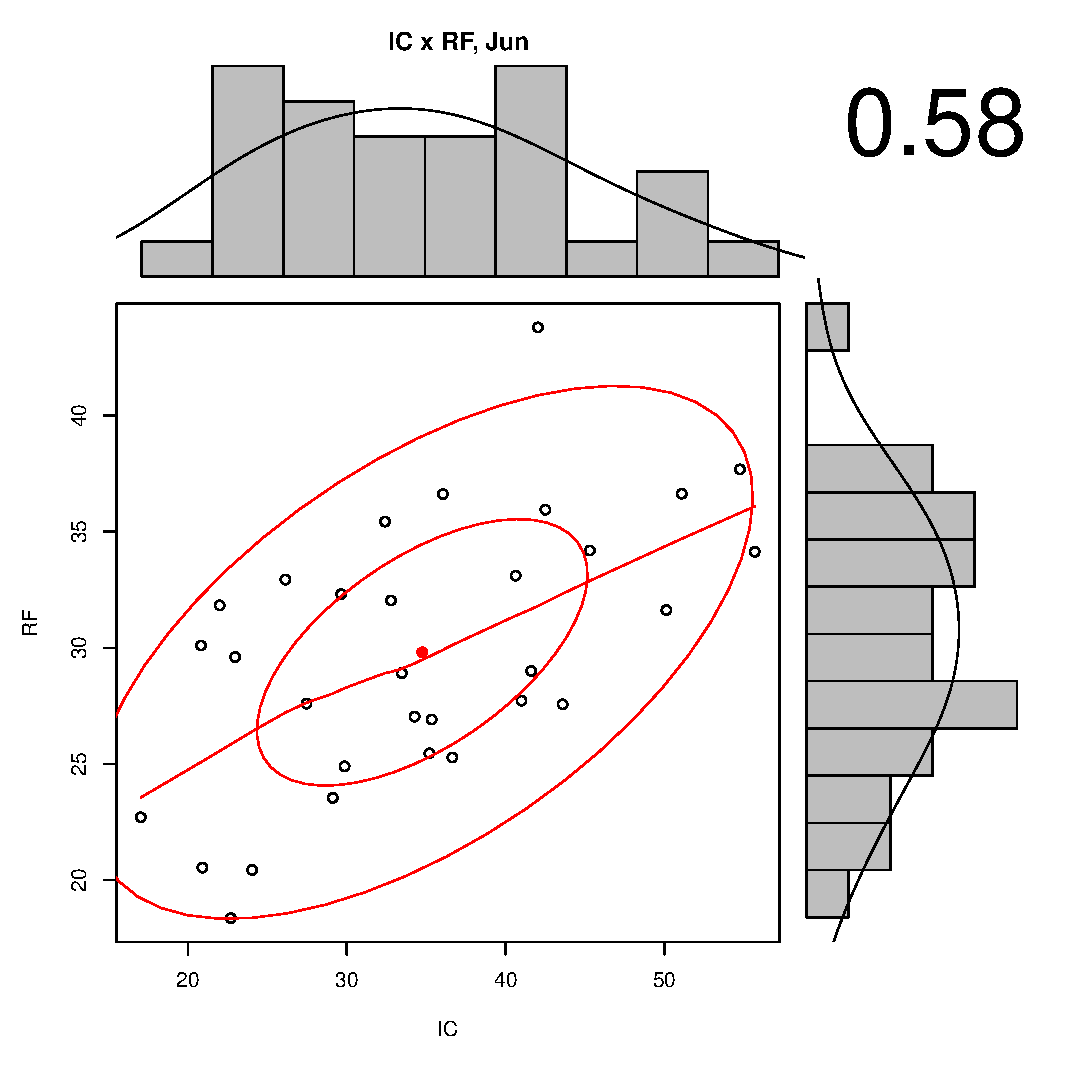
\includegraphics[height=2cm,width=2cm]{figures/HIST_ICxRF_mesJun.eps}
%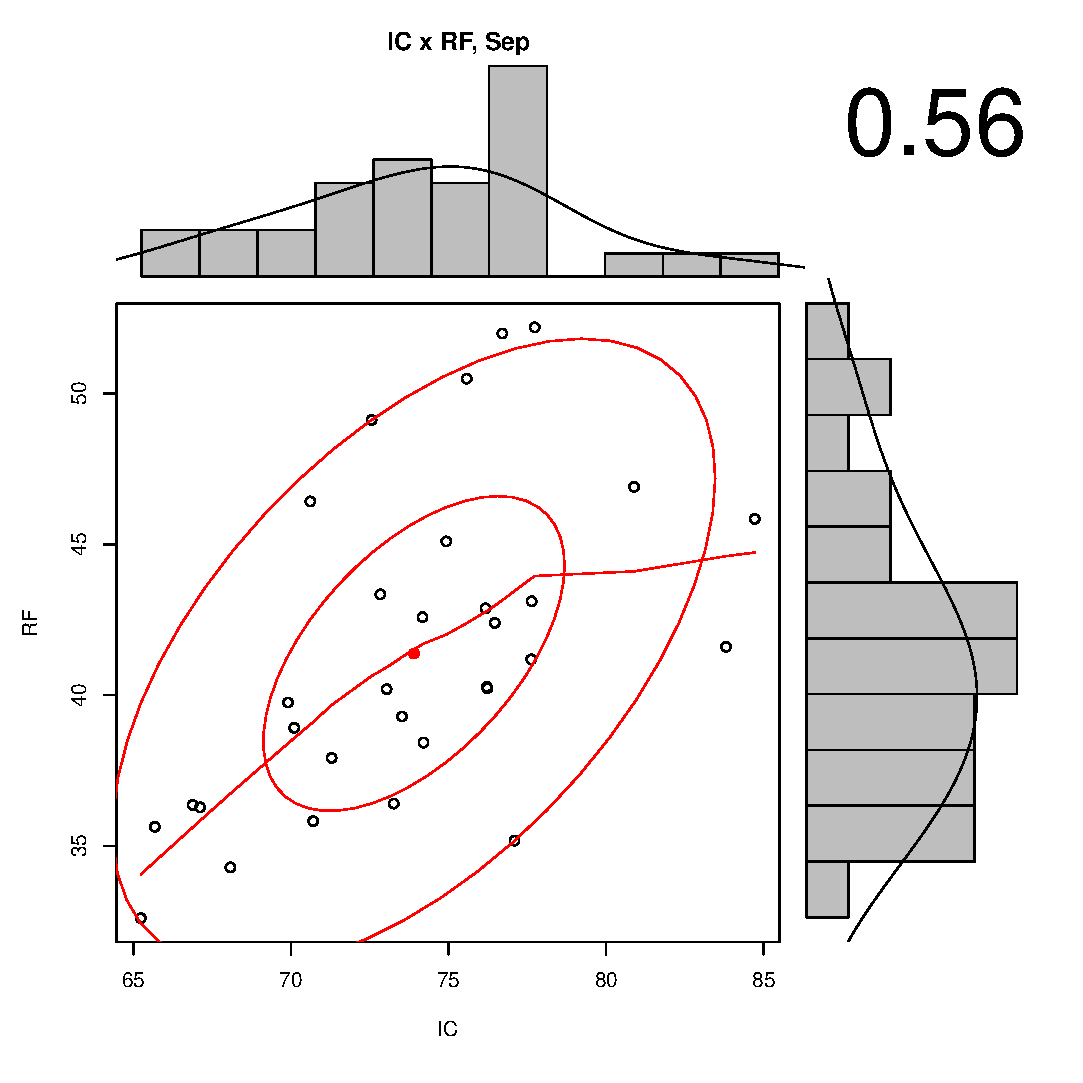
\includegraphics[height=2cm,width=2cm]{figures/HIST_ICxRF_mesSep.eps}
%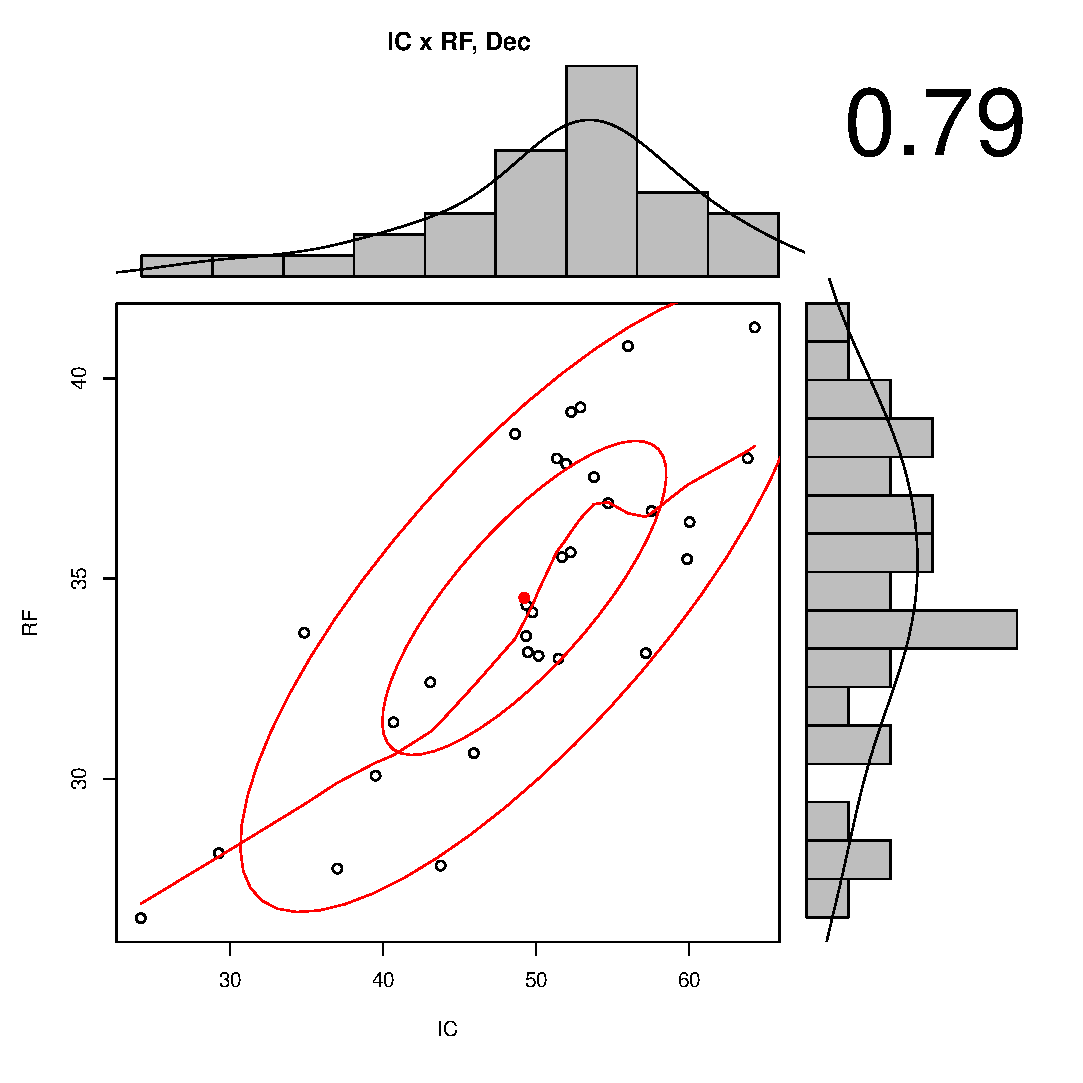
\includegraphics[height=2cm,width=2cm]{figures/HIST_ICxRF_mesDec.eps}
%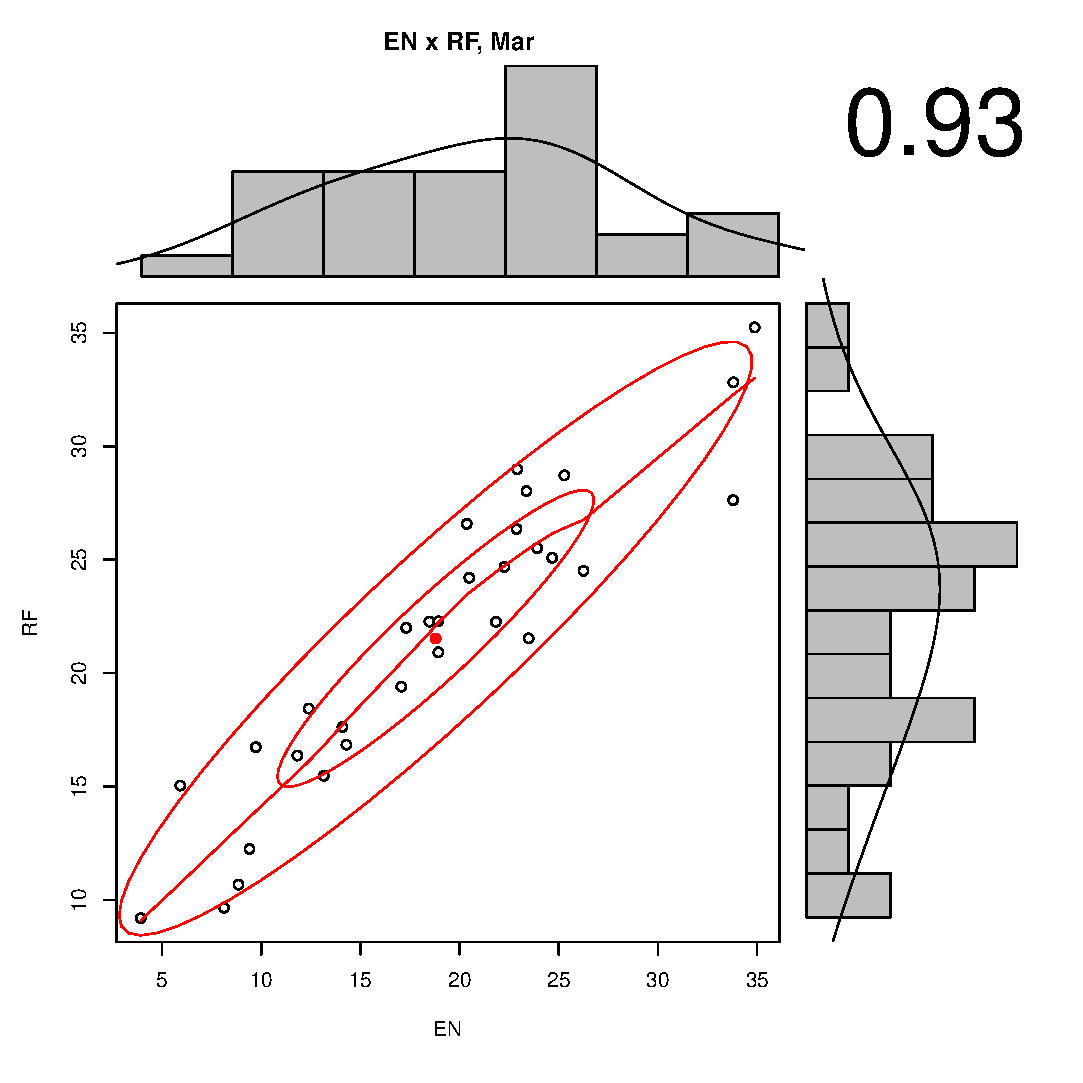
\includegraphics[height=2cm,width=2cm]{figures/HIST_ENxRF_mesMar.eps}
%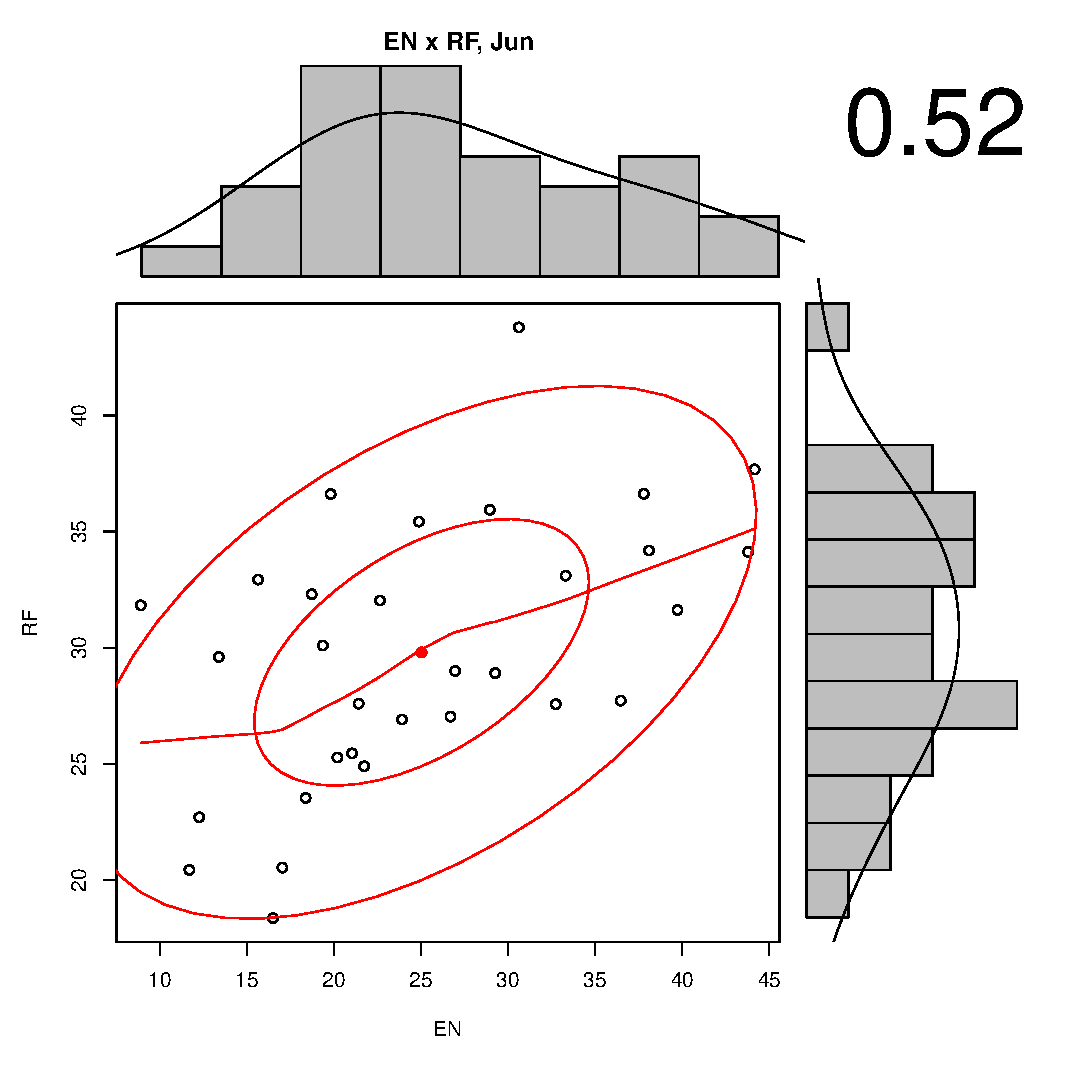
\includegraphics[height=2cm,width=2cm]{figures/HIST_ENxRF_mesJun.eps}
%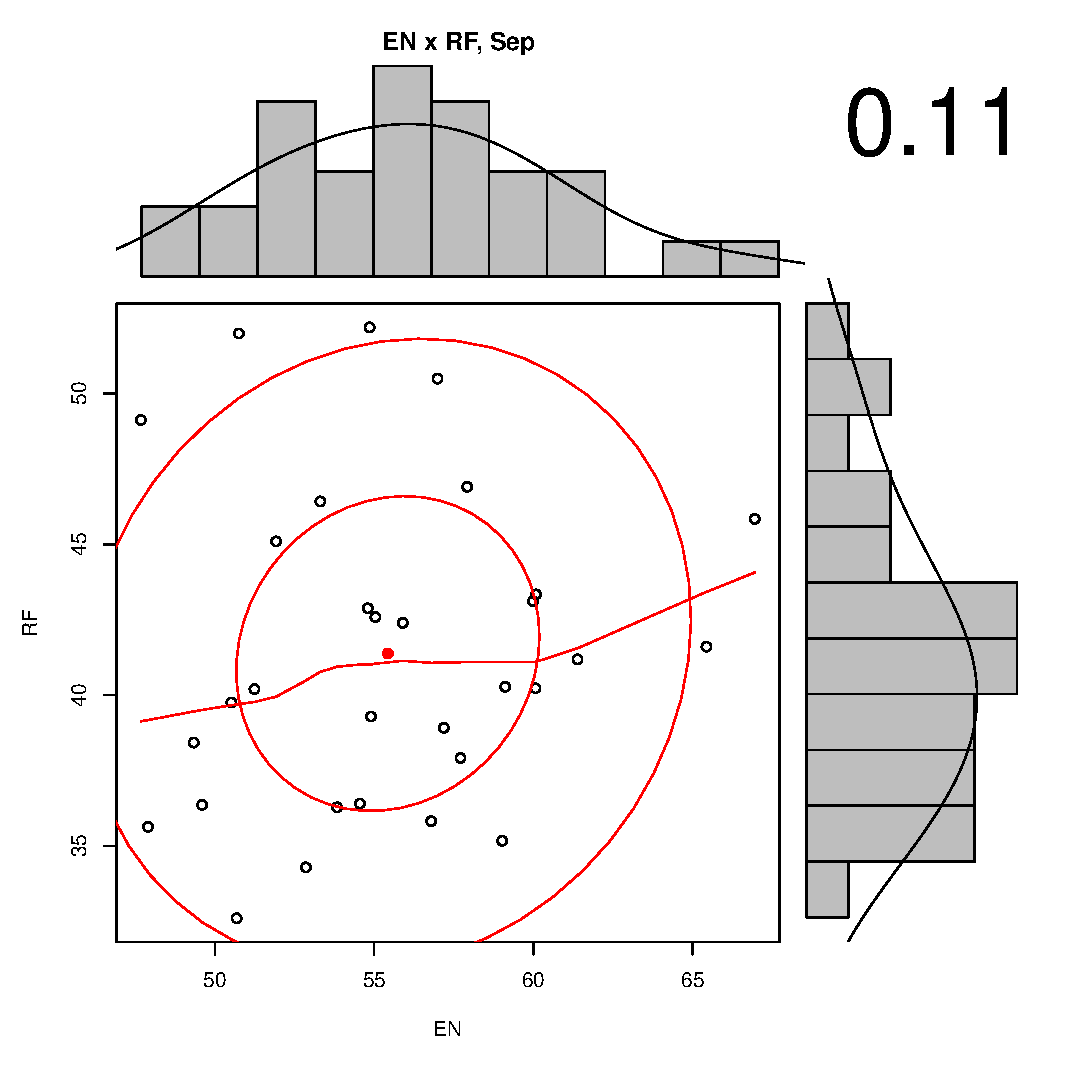
\includegraphics[height=2cm,width=2cm]{figures/HIST_ENxRF_mesSep.eps}
%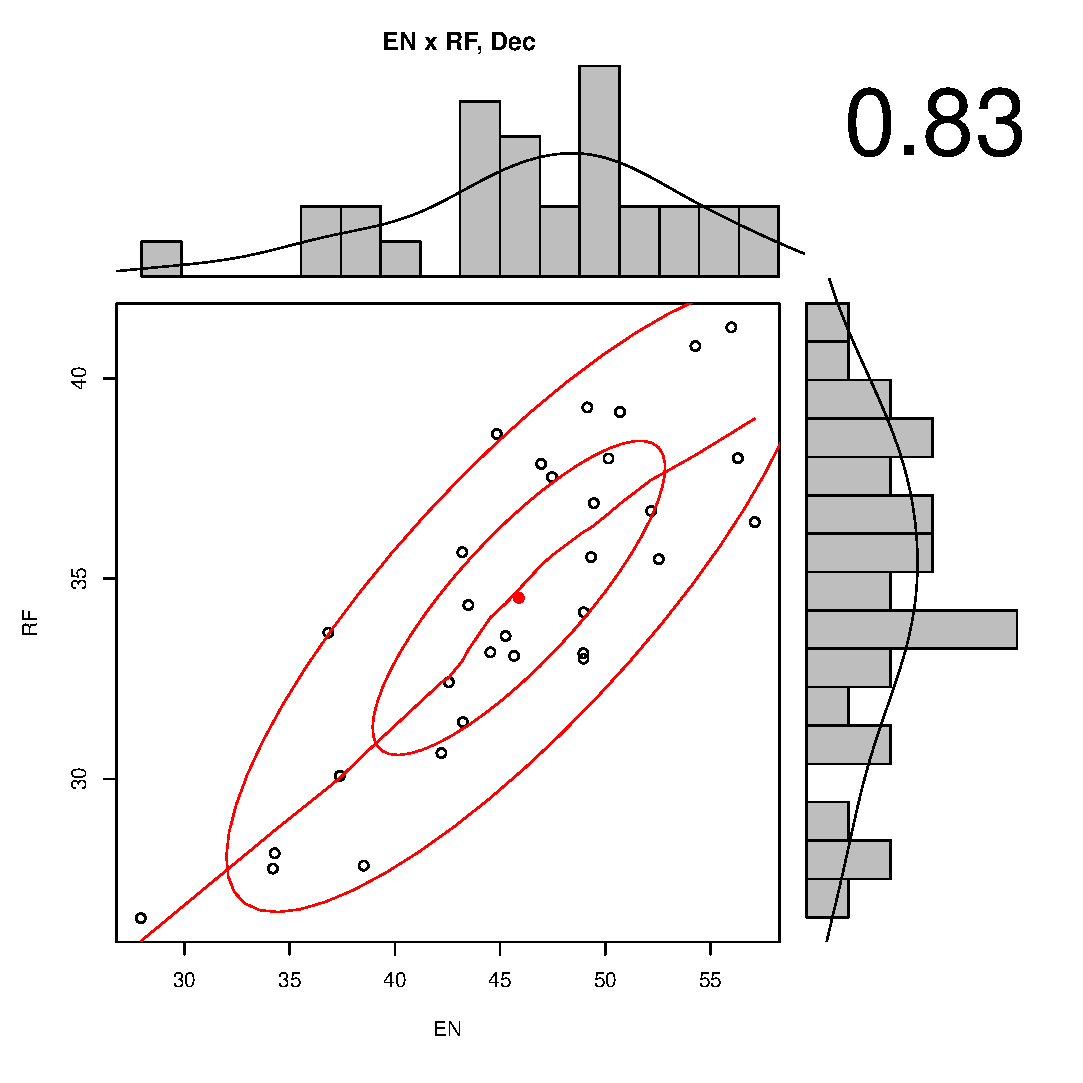
\includegraphics[height=2cm,width=2cm]{figures/HIST_ENxRF_mesDec.eps}
%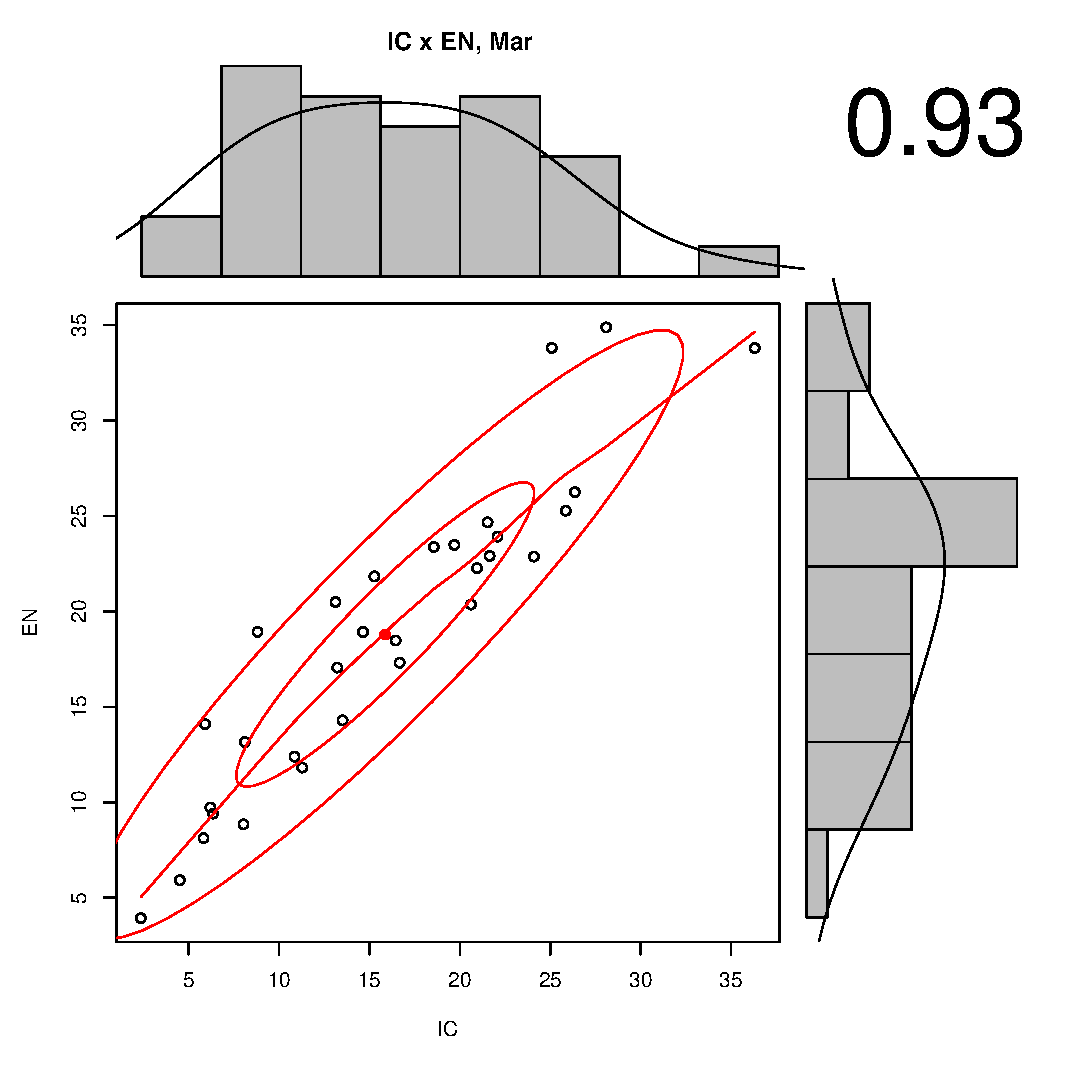
\includegraphics[height=2cm,width=2cm]{figures/HIST_ICxEN_mesMar.eps}
%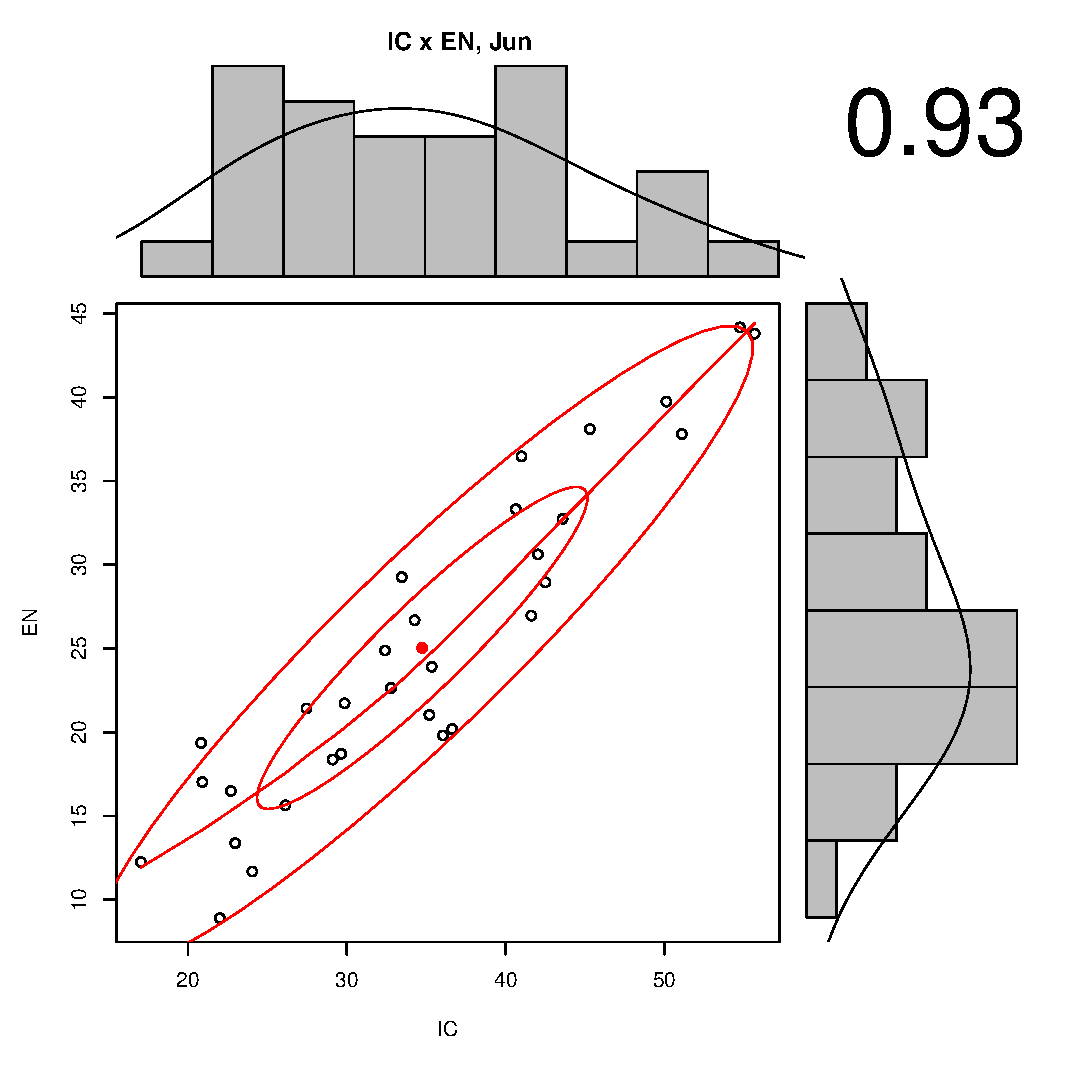
\includegraphics[height=2cm,width=2cm]{figures/HIST_ICxEN_mesJun.eps}
%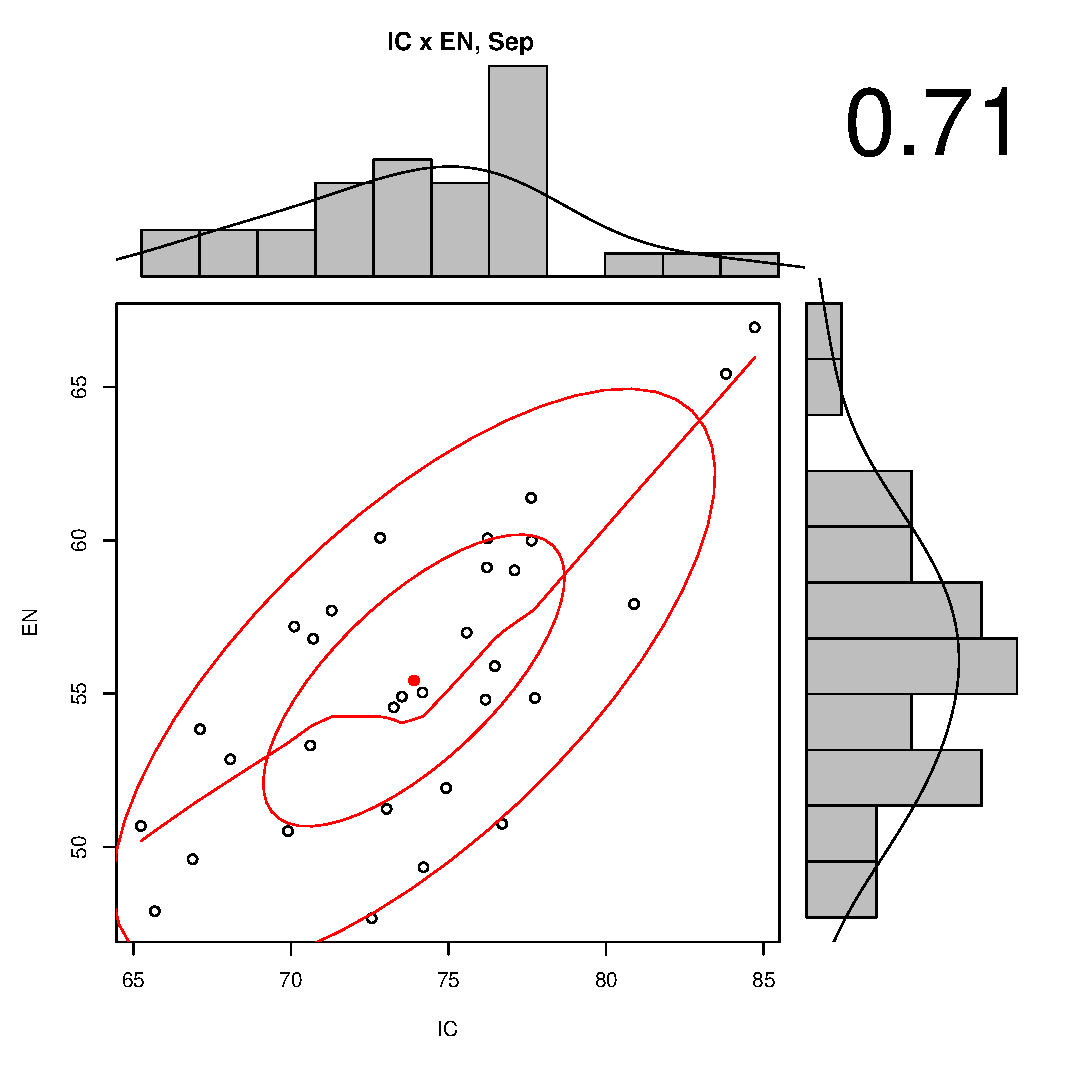
\includegraphics[height=2cm,width=2cm]{figures/HIST_ICxEN_mesSep.eps}
%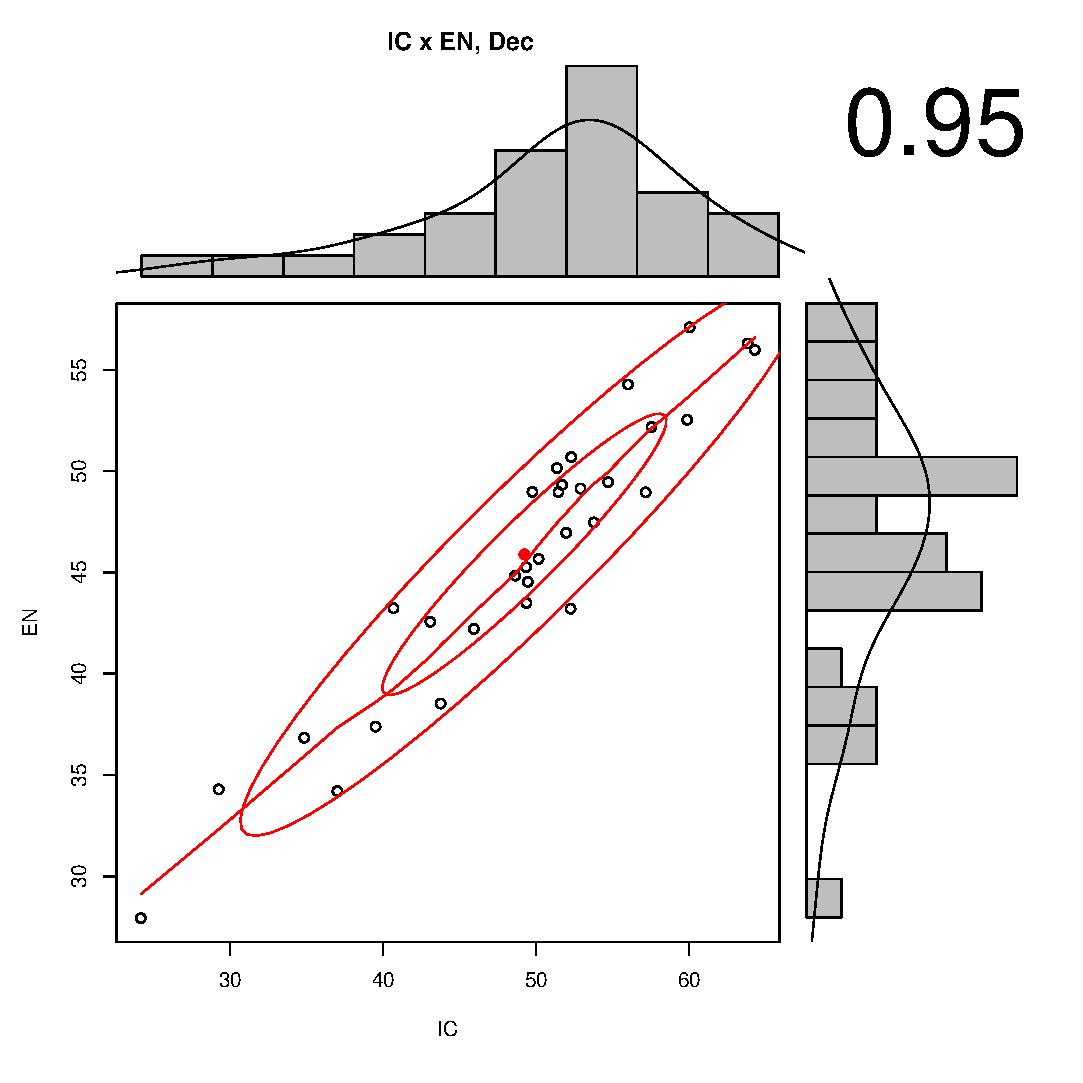
\includegraphics[height=2cm,width=2cm]{figures/HIST_ICxEN_mesDec.eps}
%\caption{Montly Histogram + Scatterplot}
%\label{hist_Scatter}
%\end{figure}




%\begin{figure}[htbp]
%\centering
%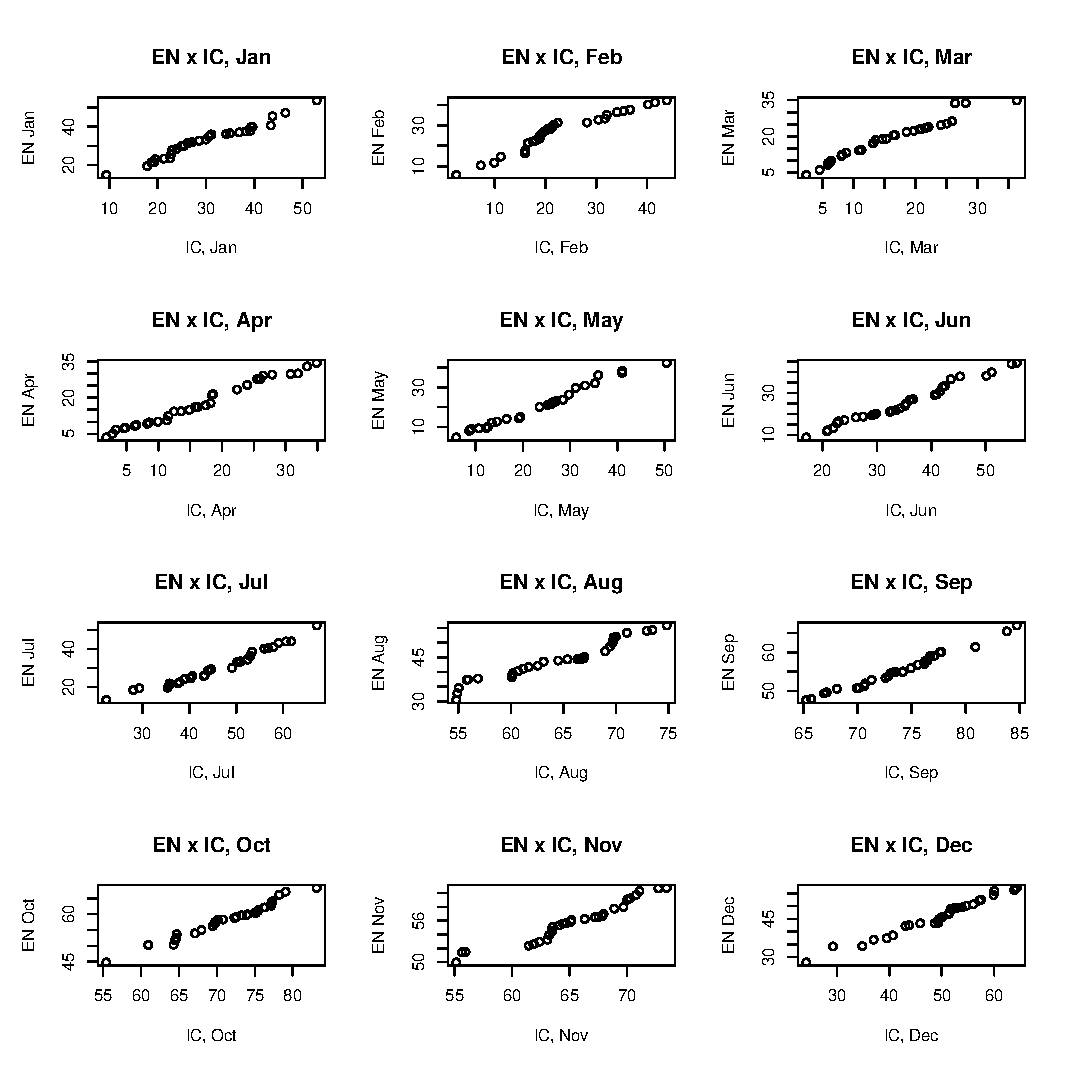
\includegraphics[height=10cm,width=9cm]{figures/ENxIC_MES.eps}
%\caption{Monthly qqplot ENxIC.}
%\label{BoxPlots}
%\end{figure}
%
%\begin{figure}[htbp]
%\centering
%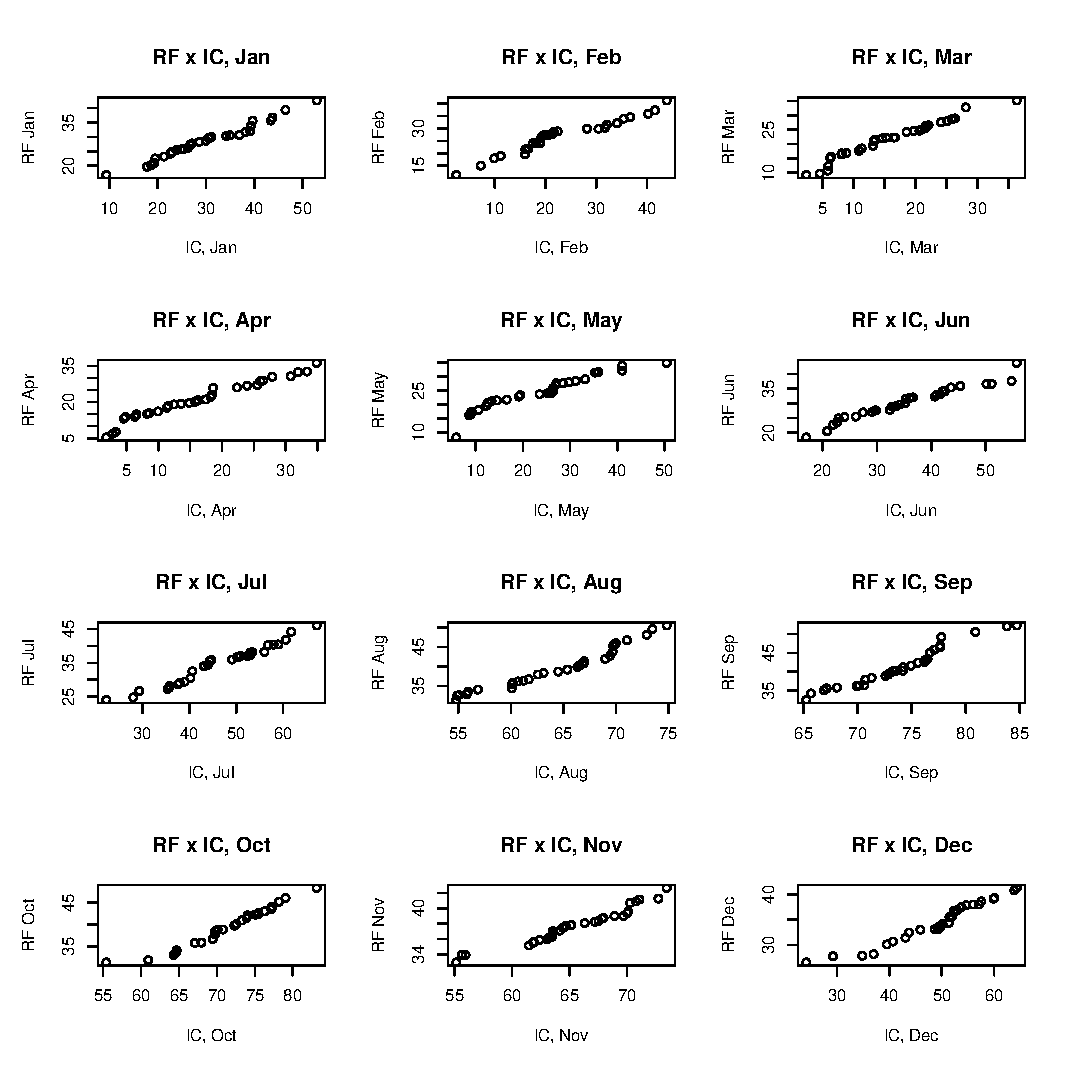
\includegraphics[height=10cm,width=9cm]{figures/RFxIC_MES.eps}
%\caption{Monthly qqplot RFxIC.}
%\label{BoxPlots}
%\end{figure}
%
%\begin{figure}[htbp]
%\centering
%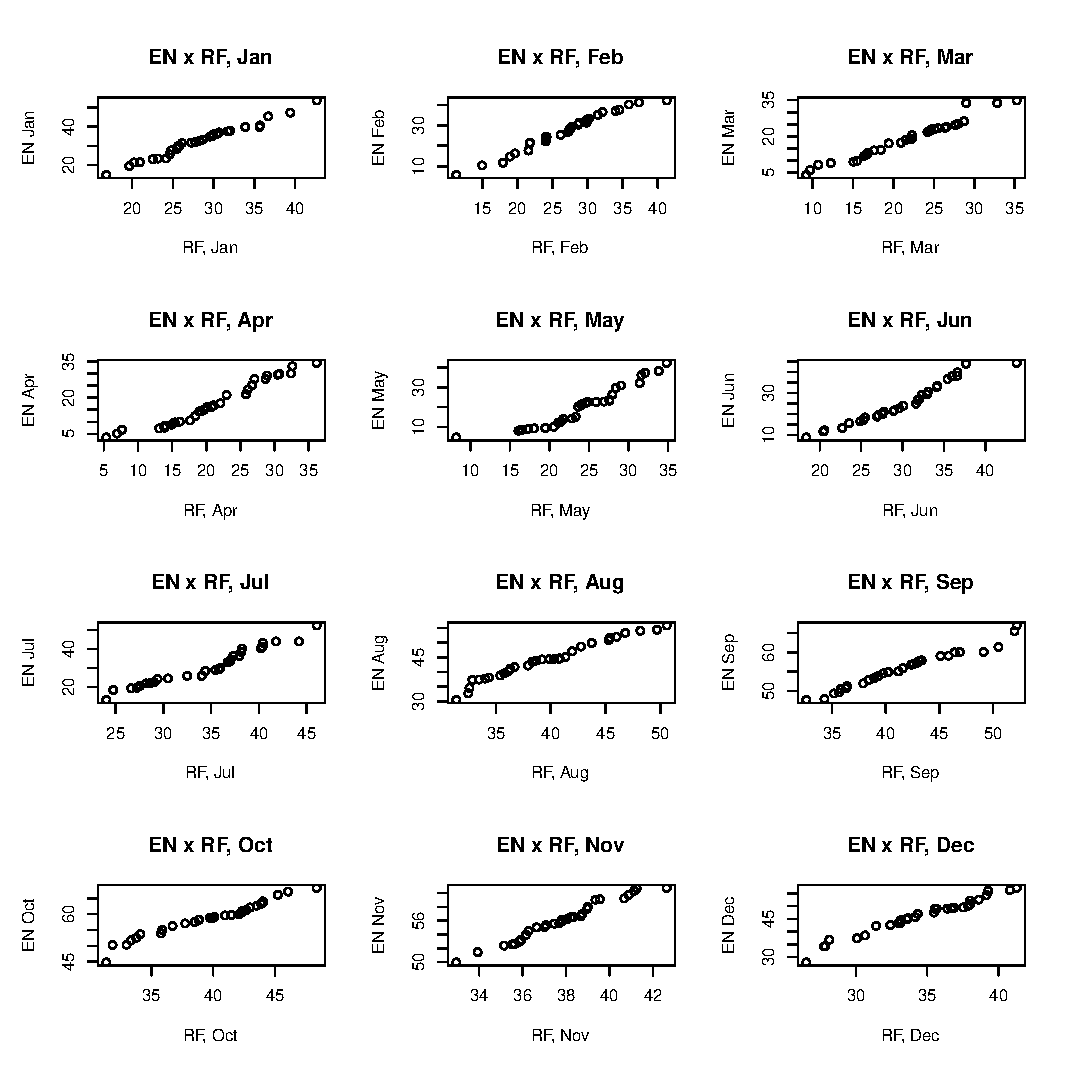
\includegraphics[height=10cm,width=9cm]{figures/RFxEN_MES.eps}
%\caption{Monthly qqplot RFxEN.}
%\label{BoxPlots}
%\end{figure}
%
%\begin{figure}[htbp]
%\centering
%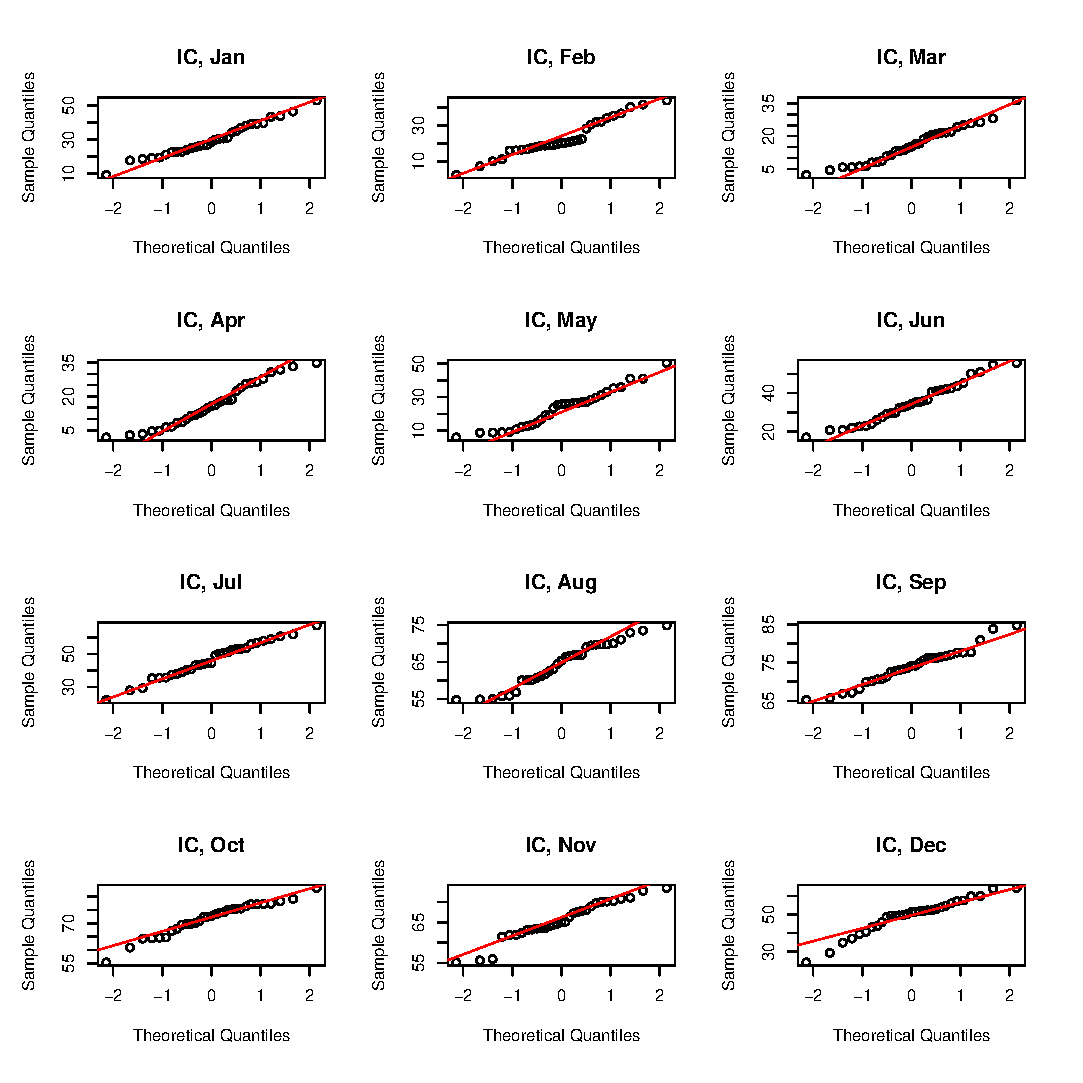
\includegraphics[height=10cm,width=9cm]{figures/IC_QQ_MES.eps}
%\caption{qqplot IC}
%\label{BoxPlots}
%\end{figure}
%
%
%\begin{figure}[htbp]
%\centering
%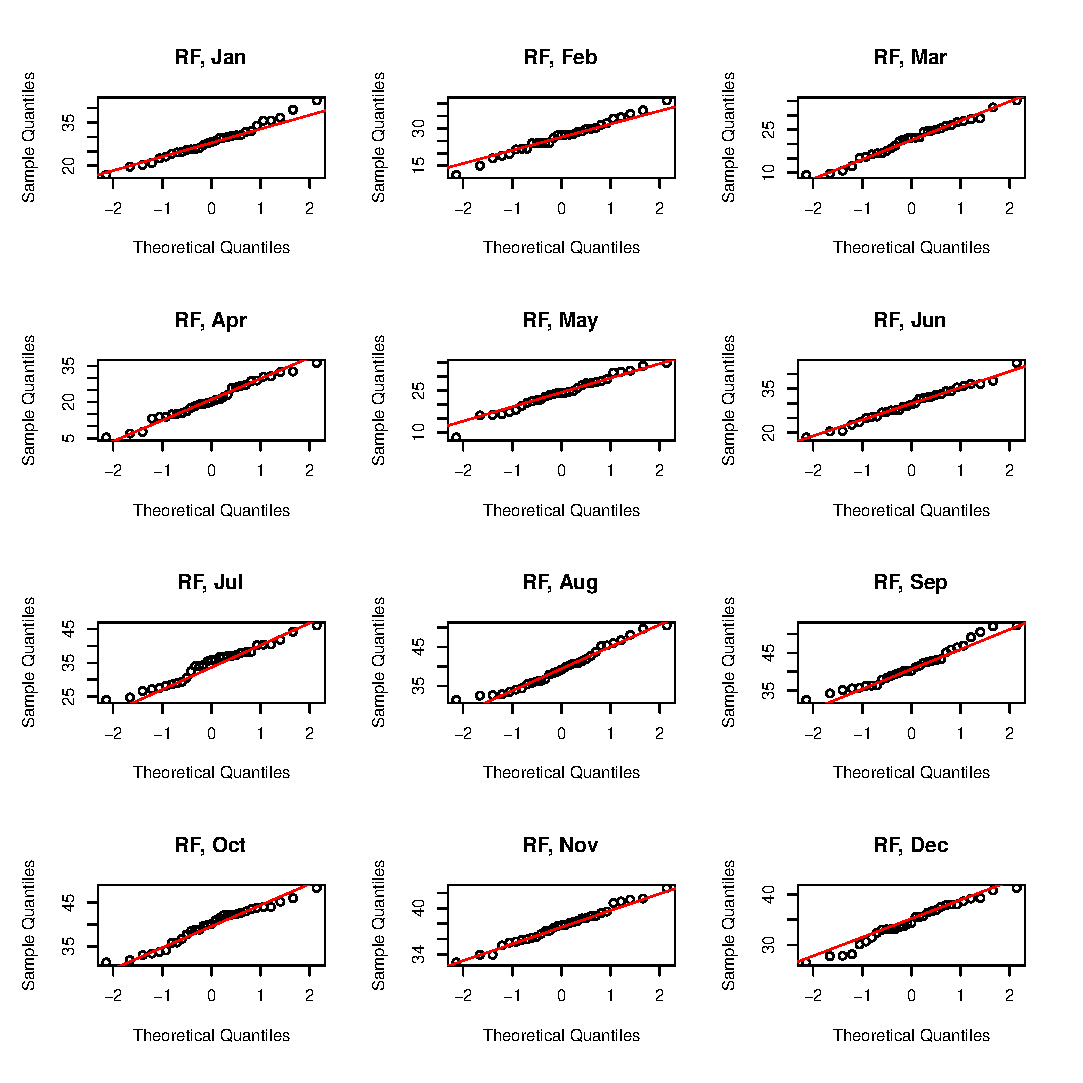
\includegraphics[height=10cm,width=9cm]{figures/RF_QQ_MES.eps}
%\caption{qqplot RF}
%\label{BoxPlots}
%\end{figure}
%
%\begin{figure}[htbp]
%\centering
%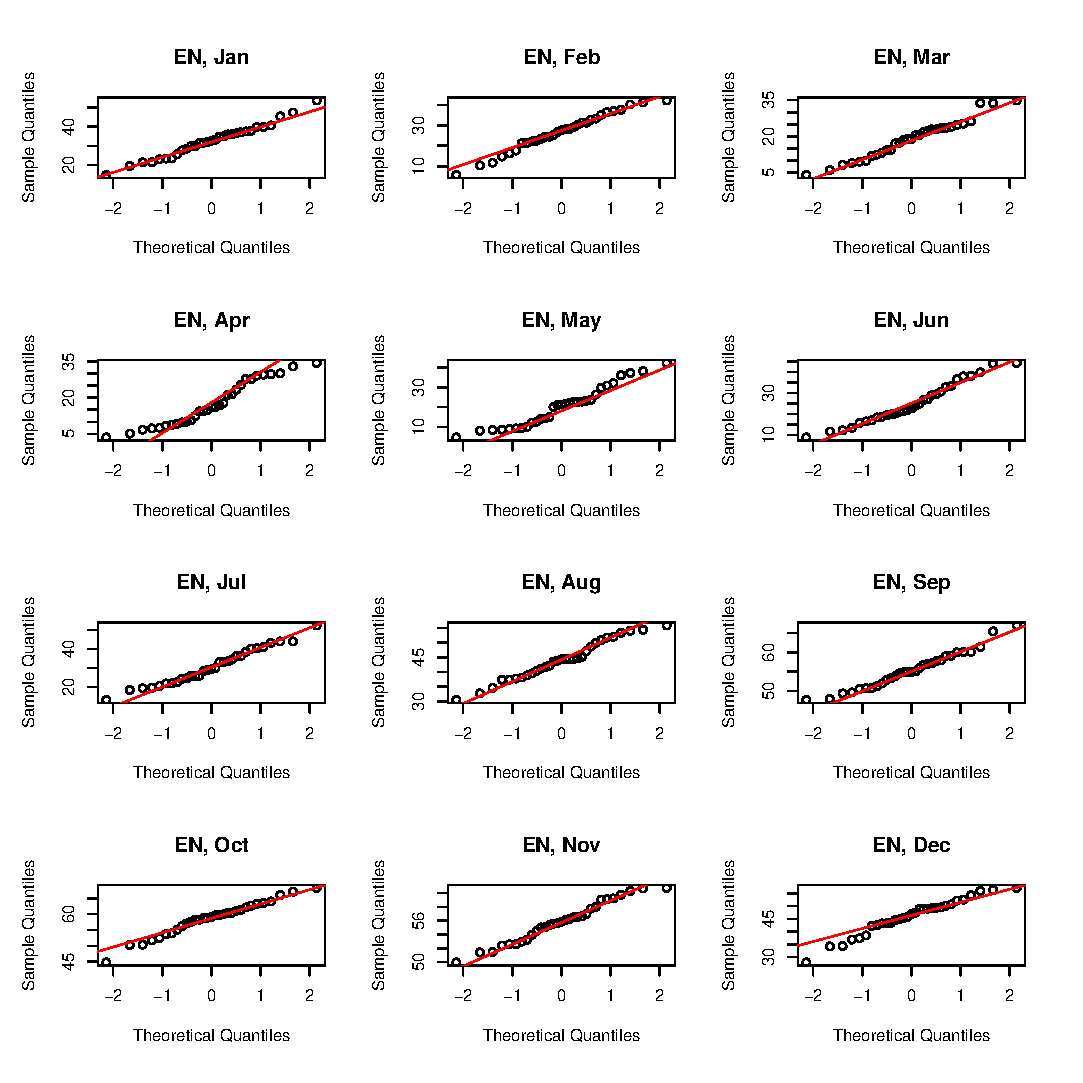
\includegraphics[height=10cm,width=9cm]{figures/EN_QQ_MES.eps}
%\caption{qqplot EN}
%\label{BoxPlots}
%\end{figure}

%\begin{table}[ht]
%\centering
%\caption{P-values of Jarque Bera test of Normality applied to each month time series.}
%\begin{tabular}{rrrrr}
%  \hline
% & Mar & Jun & Sep & Dec \\ 
%  \hline
%  IC & 0.63 & 0.57 & 0.91 & 0.13 \\ 
%  RF & 0.82 & 0.96 & 0.46 & 0.58 \\ 
%  EN & 0.82 & 0.45 & 0.60 & 0.42 \\ 
%   \hline
%\end{tabular}
%\end{table}

%In addition to the strong seasonal pattern presented by Figure \ref{BoxPlots_IC_mensal}, another important stylized fact of CF time series is provided, season effects. During the first half of the year, wind speed tends to decrease and also its frequency. As an outcome, the CF of these months will naturally drop. On the other hand, during the second semester, the opposite happens.




%and the non Gaussian pattern of such variable, which is statistically confirmed by the
%Another evidence, which corroborates with our Moreover, checking each month empirical density, it is possible to conclude that they are asymmetric, and when calculating theirs values, August`s skewness is the closest to zero, in modulus, with a value of 0.1306.

%Tradicionalmente, tem-se utilizado modelos ARMA e seus derivados, os quais pressupoe a hipotese de normalidade da serioe, o que contraria os fatos estilizados ja elucidados. Mesmo trabalhando com o log da serie, problemas persistem, pois como o objetvio é a simulacao na escala original da série, observa-se que ao se aplicar a exponenciacao, as simulacoes da serie obtida pelo modelo arma gaussiano, a magnitude dos valres simulados muitas vezes sao superiores aos valores historicamente observados

%The non Gaussian nature of CF time series, in most applications in the energy literature, is not directly dealt with, either because of non availability of proper software or by the computational burden in implementing existing non Gaussian models. For example, if one decides to fit a non-Gaussian state space model using unobserved components, such as trend, seasonals and cycle, it would be necessary extensive Monte Carlo simulation for both state and fixed parameter estimation. See, for example, Durbin and Koopman (2012, pp 209-324). In practice a great deal of applied work involving scenario generation for wind speed or CF time series make use of ARMA models and its extensions, \cite{box1976time}, mostly under normality assumption. At best such models are fitted to the log of the variable of interest, and by taking the anti log, predictions and simulations on the original scale of the variable are obtained. Unfortunately such a strategy can result in unrealistic sampling paths for the original variable.

%Hence, the need to apply the $log$ transformation and then fit the data properly. Yet, it is also a non conventional form, as it is known, to come back to the original scale, it is necessary the exponentiation of simulated Gaussian values that can result in unrealistic sampling paths as can be seen in Figure \ref{SARIMA_COM_TRANS} where we simulate 2000 scenarios 12 steps ahead.




%, and by propagation, this can badly affect the risk measures obtained from the simulated distribution of the cash flows associated with a particular portfolio of wind plants. %our approach can generate scenarios in just one step, avoiding the need of transforming back the outcome variables to its original scale, as it is the case under a Gaussian assumption for the marginal models. As it is known, exponentiation of simulated Gaussian values can result in unrealistic sampling paths for the wind capacity factor. 

%Isso cria uma motivacao para o estabelecimento de modelos que sejam capazes de modelar series nao gaussianas e que contemplem a questao de nao linearidade

%Such features motivates the insertion of a recently proposed time series framework which gracefully handles with the two aforementioned challenges. In this paper we applied to monthly  wind capacity factor (CF) time series a newly proposed class of observation-driven time series models, the so called GAS models \cite{creal2013generalized} or Dynamic Conditional Score (DCS), following \cite{harvey2013dynamic}. Our approach fits in the classification proposed by \cite{zhang2014review} as a long-term parametric probabilistic. More specifically one can pick any desirable predictive distribution judged appropriate for the response variable being modelled and, trough the dynamic equations proposed in the GAS frameworks, make its parameters time varying. We advocate that wind probabilistic forecasting should be preferred in practice since from it, apart from conditional measures of location, like mean or median, one can obtain many different measures of interest, like conditional quantiles, enabling improved decision making to power systems operators and investors.

%However, for several applications, such as unit commitment, regulation and commercialization, these variables are plugged into the power curve to transform wind speed/wind power into a CF time series. The models here proposed are directly fitted to the CF time series which are directly available, and as consequence  no such transformations will be needed. \cite{zhang2014review} presents a detailed review of state-of-the-art methods and new developments in wind power uncertainty forecasting. 
%As \cite{mur2010variability} conclude, wind power generation is a non-linear and non-stationary process, which are also features of wind speed time series. Therefore common choices of models that could reproduce its pattern use time series models (e.g. \cite{brown1984time}) or Artificial Intelligence \cite{sideratos2012probabilistic}. 

In contrast to the main objective of WPG simulation methods, which aim to produce scenarios that characterize all the conditional density and its fit to the observed quantile data, much research has been devoted to devise short-term forecast methods for wind speed and WPG time series (for instance, see \cite{zhang2014review}). In some applications on medium and long-term forecast, the time series model is conducted using conventional ARMA models with seasonal lags, or SARIMA models, under a Gaussian distribution (see \cite{souto2014high} for a high-dimension estimation process based on LASSO). In its original formulation, SARIMA models present a fixed conditional variance. To add extra flexibility to these models \cite{lau2010approaches} proposes an ARIMA model with GARCH effect, allowing the conditional variance of the WPG distribution to vary over time. Also, to provide a description of the spatial correlation of wind-speed time series, \cite{taylor2009wind} proposed an Autoregressive Fractionally Integrated-GARCH model (ARFIMA-GARCH). In these and other models, conditional on the past, the distribution of the response variable is assumed Gaussian.

The non-Gaussian nature of WPG time series is well reported in the literature (see \cite{bessa2012time,jeon2012using,taylor2015forecasting,Wan2017} and references therein). However, only very limited classes of non-Gaussian time-series models are available for modeling WPG. The state of the art literature on short-term probabilistic modeling of WPG time series mainly rely on non-parametric models. For instance, in \cite{bessa2012time} and \cite{Wan2017}, non-parametric approaches were devised to forecast conditional distributions. While in \cite{bessa2012time} kernel density estimators were employed to build a predictive conditional density function, in \cite{Wan2017} a quantile-regression-based model was used. Despite the virtues found in nonparametric methods, those models require a lot of data to be fitted and are mainly devised for the univariate case. Thus, the development of new parametric models capable to properly characterize the full multivariate non-Gaussian distribution for WPG time series is a relevant research theme, which did not received too much attention so far. Relevant applications arise from risk assessment in both medium and long-term planning/investment studies, which mainly rely on few data points to characterize conditional estimates of extreme quantiles \cite{FosteringWPP,SHAPIRO2013,Fanzeres2015,Aderson2017,kariniotakis2017renewable}.

In \cite{creal2013generalized} and \cite{harvey2013dynamic}, a general framework for time series models with time-varying coefficients was proposed considering any non-Gaussian conditional distribution, either discrete or continuous, univariate or multivariate. Such model has been named in the recent literature as Generalized Autoregressive Score (GAS) model \cite{creal2013generalized} and Dynamic Conditional Score (DCS) \cite{harvey2013dynamic}. In \cite{creal2013generalized}, it has been shown that several well-known time-series models from the econometric literature are a particular case of GAS models\footnote{For instance, GARCH models that deal with heavy tailed distributions in finance \cite{engle1986modelling}, Autoregressive Conditional Duration models \cite{engle1998autoregressive} to tackle asymmetric distributions in finance applications such as time duration, and the Poisson count models of Davis \cite{davis2003observation} are particular cases of GAS models.}. More specifically, a GAS model is built based on a user-defined conditional probability function whose parameters follow a data-driven dynamic equation, generally on the form of an autoregressive mechanism. Then, by construction, time-varying parameters can be accommodated according to an updating mechanism that uses the score as its driving force. The use of the score function for updating time-varying parameters is an intuitive choice. It is defined as the steepest ascent direction (gradient) for improving the local fit of the model in terms of likelihood. In such an updating mechanism, information from the whole density is used to track the evolution of time varying parameters. 

Most of the applications using GAS models have been published in the recent literature of finance and economics. We refer the interested reader to the main on-line repository on GAS papers \cite{GASwebpage}. The virtue of GAS models to address non-linear and non-Gaussian time series notwithstanding, to the best of the authors' knowledge there is no publication in the power systems literature using such framework. The consideration of a seasonal structure in the updating mechanism for the time-varying parameters was also not addressed in the GAS literature so far, despite being a relevant structure shared by a wide range of time series such as WPG (see \cite{tseng2002fuzzy,lei2009review,FosteringWPP,souto2014high} and references therein). 

%Additionally, it is crucial to incorporate spatial dependence information when simulating multivariate scenarios in applications involving many different generation units \cite{souto2014high}, e.g. unit commitment, energy trading, just to mention a few. %More commonly, such dependence is usually captured by the covariance matrix $\Sigma$ \cite{pinson2009probabilistic}. For example, \cite{morales2010methodology} uses a multivariate ARMA model and employed the variance-covariance matrix to characterize the spatial-temporal correlation of wind speed distribution. 
%In our approach, the dependence structure among the WPG time series for different power plants will be captured through an elliptical copula applied to the residuals of the univariate GAS models. In order to allow the consideration of a time-varying spatial dependence, the copula parameter will be updated by a GAS mechanism, similar to \cite{creal2011dynamic}. Copula-based models are very flexible to construct multivariate distributions, since they allow the specification of the models for the marginals distributions (in our case the beta GAS models) separately from the dependence structure given by the copula.
%Details on estimation and inference for copulas applied to time series can be found in \cite{cherubini2004copula,joe2005asymptotic, patton2012copula, patton2009copula, patton2006modelling, patton2002applications}. %The adoption of a time-varying correlation matrix for the copula is needed to incorporate the different spatial-dependence regimes observed along seasons \cite{souto2014high,vecchia1985maximum}.% In our set up the correlation matrix will also evolve in time according to a second step GAS procedure as presented in \cite{creal2011dynamic}%, which will makes it easier to capture and correct for outlier effects.

To generate joint scenarios for WPG time series based on GAS models for power plants belonging to different geographical areas, it is important to include spatial dependence information among these units \cite{souto2014high}. In \cite{creal2011dynamic}, the authors provided an empirical application for a panel of daily-equity returns updating both variance and correlation matrix by the proposed GAS mechanism for a multivariate Student t density function. They indicate the link between their framework to a time-varying copula specification, but no results and tests were provided. %The key is the implementation of the matrix $\Psi_t$ and the time varying vector $f_t$ which will be presented latter in this section. 
Furthermore, it is possible to combine linear models with copulas that also have time-varying parameters as shown in \cite{patton2006modelling,patton2009copula,patton2012copula}. However, none of such works proposed a GAS mechanism to update time-varying parameters from both marginal densities and copula structures. 

The objective of this paper is to propose a new methodology to address non-Gaussian WPG multivariate time-series through GAS models. We also propose a time-varying copula-based approach to capture the dynamics of spatial dependencies. Therefore, the contribution of this paper are twofold:

\begin{itemize}
	\item A new simulation framework based on GAS models capable to generate non-Gaussian joint scenarios for multivariate WPG time series. The proposed framework allows the simulation of non-Gaussian scenarios widely demanded in many power system applications such as planning, operation, and risk assessment.
	
	\item A new spatial-dependency method for GAS models through a time-varying elliptical copula model applied to the residuals of the univariate GAS models. In our proposed framework, the copula parameter, namely, a correlation matrix, is guided by a novel second GAS mechanism allowing the consideration of a spatial-dependence structure that changes along seasons. This is a significant step forward on the subject of modeling GAS models that allows a good characterization of multivariate WPG time series where all these effects are found. Thus, in our proposed framework, both time and spatial dependences are guided though GAS-based updating mechanisms.
\end{itemize}

The rest of this paper is organized as follows. In section \ref{marginals}, the proposed univariate GAS model framework with seasonal dynamics in the updating mechanism is presented. Estimation, diagnoses, and forecast procedures are also discussed in this section. In section \ref{copula}, an elliptical-copula model is devised based on \cite{creal2011dynamic} to model the time-varying correlation matrix for the residuals. In section \ref{Application}, a case study using realistic data from the Brazilian power system is presented to illustrate the application of the proposed framework. Finally, in section \ref{Conclusion} conclusions are addressed.

% ========== ========== ========== ========== ========== 
% ===== Sec. II - Marginal Models ===== %
% ========== ========== ========== ========== ========== 

\section{GAS models} \label{marginals}

We consider a generic normalized WPG time series with a support in the range [0,100), in percentage of the maximum power injected. The densities selection rely on the support range and shape of conditional distributions. In this work we select and study the case of a Beta distribution with the first-shape parameter varying over time. More precisely, in our application, the $i$-th, from a set of $K$, WPG time series is described by a beta probability density function (PDF) as follows:

\begin{equation}
p(y_{it}|f_{it},\mathcal{F}_{i,t-1};\theta_i) \sim beta\left(\beta_{it},\alpha_{i}\right) \forall\,\, i \in K \,\, \mbox{and}\,\, t \in T, \label{beta_dens}
\end{equation}

\noindent
where $y_{it}$ is the WPG injected by unit $i\in K$, at time $t$, $f_{it}$ is generally defined as a logarithmic transformation of the time-varying first shape parameter of the beta distribution, $\beta_{it}$, to avoid nonnegativity constraints in the estimation process, and $\alpha_i$ is the second shape parameter, in this paper assumed to be fixed. $\theta$ is the vector of hyperparameters, assumed to be static in time, encompassing $\alpha_i$, dummy variables to capture the effect of outliers when needed, and the rest of parameters to be estimated.

Thus, the time-varying parameter GAS$(p,q)$ updating mechanism is devised for $f_{it}$ as follows:

\vspace{-0.3cm}
\begin{equation}
{f}_{i,t+1} = \omega_i + \sum_{l=1}^{p} A_{i,l}s_{i,t-l+1} + \sum_{l=1}^{q} B_{i,l}f_{i,t-l+1}. \label{eq:2}
\end{equation}

\noindent
In expression \eqref{eq:2}, $s_{i,t-l+1}$ is the score of the beta PDF for unit $i$ at time $t-l+1$, and $\omega_i$, $A_{i,l}$, and $B_{i,l}$ are fixed parameters, which are considered as part of vector $\theta_i$. %Thus, in this work, $\theta = [\textbf{A}_i,\textbf{B}_i,\omega_i]^T$, where $\textbf{A}_i$ and $\textbf{B}_i$ stand for the vector contain all lags of $A_{i,l}$ and $B_{i,l}$ fixed parameters.

To complete the description of the the updating mechanism of GAS models it is necessary to define $s_{i,t}$ in  Equation \eqref{eq:2}. The authors in \cite{creal2013generalized} proposed the following scheme:
\begin{align}
s_{i,t} &= \mathcal{I}_{i,t|t-1}^{-d} \cdot \nabla_{i,t}\label{eq:score1}\\
\nabla_{i,t} &= \frac{\partial \ln p(y_{i,t}|f_{i,t},\mathcal{F}_{i,t-1};\theta_i)}{\partial f_{i,t}}\label{eq:score2}\\
\mathcal{I}_{i,t|t-1} &= E_{t|t-1}[\nabla_{i,t}^{T}\nabla_{i,t}],\label{eq:score3} 
\end{align}
\noindent
where $p(y_{i,t}|f_{i,t},\mathcal{F}_{i,t-1};\theta_i)$ is the observation PDF, $\mathcal{F}_{i,t-1}$ collects all relevant information of time series $i$ up to time $t-1$, and $\mathcal{I}_{i,t|t-1}$ is a scaling factor, which accounts for the variance of $s_{i,t}$. More details can be found in \cite{creal2013generalized}. In practice, the choice of $d$ has shown to be an empirical question: for a given model one chooses the value of $d$ which produces best diagnostics and forecasting.

As mentioned before, because the beta parameter can only assume positive values, it is conveniently reparameterized as the exponential of an unconstrained parameter, namely, $f_{i,t}$. In addition, to remove the effect of possible outliers, dummy variables can be considered into parametrization. In this sense, if we define the time-varying beta parameter as 
\begin{equation}
\beta_{i,t} = e^{\phi_i^T D_{i,t} + f_{i,t}}, \label{eq:exogena}
\end{equation}

\noindent
with
\begin{equation}
D_{i,t}=
\begin{cases}
1 , & \text{if } y_{i,t} \text{ is an outlier;} \\
0,  & \text{otherwise}.
\end{cases}
\end{equation}

\subsection{Estimation} \label{MVunivariado}

Regarding the estimation of the fixed parameter vector $\theta_i$ for each time series $i$, the estimation procedure is based on the following log-likelihood maximization problem:%\footnote{We recall that the first shape parameter of the beta density, $\beta_{i,t}$, can be recovered after the estimation process by making $\beta_{i,t}=exp\{f_{i,t}\}$.}: 

\begin{equation}
\hat{\theta}_i = arg\underset{\theta_i}{max} \sum_{t=1}^{n} ln[p(y_{i,t}|f_{i,t},\mathcal{F}_{i,t-1};\theta_i)].\label{eq:max}
\end{equation}

%From this, it follows that Equations \eqref{beta_dens}-\eqref{eq:score3} should also be re-parametrized with regard to $\ln(\beta_t)$. Considering a monotonically increasing mapping function $h(\cdot)$, then $\tilde{f}_{t}=h(f_{t})$. Taking $\dot{h_{t}} = \partial h(f_{t})/f_{t}^{'}$, the beta GAS specification updating mechanism, will be
%\begin{align}
%\dot{h}_{t} &= \frac{1}{\beta_{t}}\nonumber\\
%\tilde{\nabla_{t}}&=\beta_{t}\left\{\ln y_{t} - [\ln k + \psi_{1}(\beta_{t}) - \psi_{1}(\beta_{t}+\alpha)]\right\}\\
%\tilde{\mathcal{I}}_{t|t-1} &= \left\{ \beta_{t}^{2} [ \psi_{2} (\beta_{t} + \alpha) - \psi_{2} (\beta) ] \right\}^{-1}\\
%\tilde{s}_{t}&=\frac{\ln y_{t} - [\ln k + \psi_{1}(\beta_{t}) - \psi_{1}(\beta_{t}+\alpha)]}{\beta_{t}^{1-2d}[\psi_{2}(\beta_{t}) - \psi_{2}(\beta_{t} + \alpha)]^{1-d}},\label{betascore1}
%\end{align}
%\noindent
%where $\psi_{i}$ stands for the $i$-th order derivative of the logarithm of the gamma function.

Because $f_{i,t}$ is a function of $\theta_i$ (we recall that the coefficients in equation \eqref{eq:2} are all part of the vector of hyperparameters, $\theta_i$), to solve the estimation problem \eqref{eq:max}, a numerical non-linear optimization procedure has to be used. In this work, we apply the Nelder Mead algorithm to find good initial points to the BFGS algorithm. Notwithstanding, the evaluation of the log-likelihood function requires initial values for $f_{i,0},f_{i,-1},...,f_{i,1-q}$ and $s_{i,0},s_{i,-1},...,s_{i,1-p}$. These  are obtained by fitting fixed beta distributions, one for each month, assuming both parameters fixed in time. More precisely, the WPG time series is split into 12 monthly time series, i.e., $\{Y_{Jan}^{(i)},..., Y_{Dec}^{(i)}\}$. Then, for each of these time series $\{Y_{v}^{(i)}\}_{v=1}^{12}$, a fixed beta density is estimated  via maximum likelihood, resulting in the estimates  $\{\alpha_{v}^{(i)}\}_{v=1}^{12}$ and $\{\beta_{v}^{(i)}\}_{v=1}^{12}$. These are then used to initialize the recursion in \eqref{eq:2} for each evaluation of the log-likelihood function. Thus, the function that is passed to the BFGS algorithm is a numerical function that receives as input a trial value for vector $\theta_i$, calculates the value of $f_{i,t}$ according to expression \eqref{eq:2}, and returns as output the value of expression \eqref{eq:max}. Based on an initial value for $\theta_i$, the BFGS algorithm iterates until finding a local maximum point. To enhance the solution quality, a Nelder Mead algorithm is used on the top of this process and its solution is used as initial points for the BFGS step and it iterates until the GAP between theses solutions are smaller than 0.1.

\subsection{Diagnostics}

Diagnostics in GAS models can be obtained using an appropriate type of residuals for non linear and non Gaussian time series models known as quantile residuals. As described in \cite{dunn1996randomized}, the observed quantile residual is given by
\begin{equation} \label{residq}
r_{t,\hat{\theta}_i} = \Phi^{-1}[F(y_{i,t}|f_{i,t},\mathcal{F}_{i,t-1};\hat{\theta}_i)].
\end{equation} 

Where $F(\cdot)$ is the cumulative distribution function (CDF) associated with the proposed beta density  $p(y_{i,t}|f_{i,t},\mathcal{F}_{i,t-1};\theta_i)$ and $\Phi^{-1}[\cdot]$ is the quantile function of a standard Gaussian distribution. Under correct model specification, these residuals should be normally distributed and show no temporal dependence. These can be checked, for example, using the Jarque Bera test for normality, the Ljung Box test for absence of serial correlation, and Ljung Box (on squared residuals) to test for absence of non linear dependence, such as ARCH effect. 

%\subsection{Univariate Forecasting}
%
%The $h$ steps ahead distribution conditional on observations up to time $t$, $p(y_{i,t+h}|\mathcal{F}_{i,t} )$, is only analytic for $h=1$, when it coincides with the chosen probability model. For more than one step ahead, $h>1$, it has to be evaluated using Monte Carlo simulation.


% ===== Sec. III - Copula Model ===== %

\section{Spatial Dependence model}\label{copula}

Once the proposed beta GAS models were individually applied to each of the $K$ WPG time series, the observed dependence among different units is captured by the probability integral transformed (PIT) variables, $\mathbf{u}_{t} \in \mathbb{R}^K$, which are calculated as 
\begin{eqnarray}\label{pits}
u_{i,t}=F(y_{i,t}|f_{i,t},\mathcal{F}_{i,t-1},\hat{\theta}_{i}) \,\, \forall \,\,i \in K\,\, \mbox{and} \,\, t=13,\ldots,T.
\end{eqnarray}
\noindent
The PIT multivariate time series denoted by $\mathbf{u}_{t}$ belong to the $[0,1]$ support. 

%where $\hat{\theta_i}$ are the estimated fixed parameter vectors from each of the univariate beta GAS model. Due to initial values of the beta GAS models, $t$ starts at 13.After obtaining vector $\mathbf{u}_{t} \in \mathbb{R}^K$, the second step GAS procedure, which updates the time-varying correlation matrix $\Sigma_t$ of the residuals of the beta models, can be estimated.

Assuming $G_{\nu}$ as the CDF of a univariate Student t distribution with $\nu$ degrees of freedom, a new vector of t-Student-distributed time series can be build as follows: $\tilde{y}_{t}=[G_{\nu}^{-1}(u_{1,t}), ..., G_{\nu}^{-1}(u_{K,t})]^T$. The elliptical copula used in this work is developed under the assumption that the transformed time series, $\{\tilde{y}_{t}\}_{t\in T}$, can be modeled as a multivariate t-Student PDF given by:

\begin{align} 
\begin{split}
g(\tilde{y}_{t}|\Sigma_{t}; \nu) = \frac{\Gamma\left(\frac{\nu+K}{2}\right)}{\Gamma\left(\frac{\nu}{2}\right) [(\nu-2)\pi]^{K/2} |\Sigma_{t}|^{1/2}} \left[ 1+ \frac{\tilde{y}_{t}^{'}\Sigma_{t}^{-1}\tilde{y}_{t}}{(\nu-2)} \right], \label{eq:denstmulti}
\end{split} 
\end{align}
\noindent
where $\Sigma_t$ is the correlation matrix which is assumed to follow a second GAS updating mechanism similar to that proposed in \cite{engle2002dynamic}. The key of such model is the use of a factorization scheme for $\Sigma_t$ that allows the updating mechanism to always generate positive definite correlation matrices. Such factorization scheme, used in \cite{engle2002dynamic} and simplified here, is described in the sequel: 

\begin{align}
\Sigma_{t} = diag(Q_{t})^{-1/2}Q_{t}diag(Q_{t})^{-1/2}. \label{sigma}
\end{align}

\noindent
%In \eqref{sigma}, $D_{t}$ is a diagonal matrix of standard deviations. However regarding the context of this paper, variances are assumed to be known since in a copula specification only the correlations are time-varying, hence $D_{t}=I$, where $I$ is an identity matrix with the appropriate dimensions. 
where $Q_{t}$ is a symmetric positive definite matrix which guarantees a symmetric positive definite matrix $\Sigma_{t}$ with elements outside the main diagonal lying inside the [-1,1] range.

%and $\Delta_{t}$ is a diagonal matrix which elements are the square root of the elements contained in the main diagonal of $Q_{t}$. The matrix $R_{t}$ applies a parametrization in the matrix $Q_{t}$ which guarantees a symmetric matrix $\Sigma_{t}$, positive definite, with elements outside the main diagonal lying inside [-1,1] range. 

The matrix $Q_t$ carries all the information regarding the spatial dependence structure among different WPG time series. The idea of adopting a time varying mechanism to update the elements of $Q_t$ is to include the temporal variation of this dependence when generating joint scenarios of WPG. In order to update the quantities of the time-varying vector $q_t=vech(Q_{t})$, which stands for the half-vectorization\footnote{The half-vectorization is a linear transformation used to convert the lower triangular portion of $K\times K$ symmetric matrices in to $K(K+1)/2$ vectors.} of $Q_{t}$, we adopt the same GAS dynamic proposed in \cite{creal2011dynamic}, i.e.,
\begin{align}
vech(Q_{t+1}) &= \Omega + \Pi s_t + \Upsilon vech(Q_{t}). \label{gasmulti}
\end{align}
\noindent
In \eqref{gasmulti}, $\Pi$ and $\Upsilon$ are diagonal matrices, $\Omega$ is a $K \times 1$ vector with elements equals to one when updating the elements of the main diagonal of $Q_t$ in order to identify either model. Hence the elements of $\Omega$ corresponding to the diagonal elements of $Q_t$ can be multiplied by any arbitrary positive number without changing the decomposition. Regarding the elements of the GAS mechanism $s_t$, $\nabla_{t}$ and $\mathcal{I}_{t|t-1}^{-1}$ for the multivariate Student t distribution, they were calculated in \cite{creal2011dynamic} and can be found in Appendix \ref{FirstAppendix}.

\subsection{Estimation of the copula parameters}\label{copula_par}
We now deal with the estimation method used in the second-step GAS procedure, i.e., the estimation of the static parameters of the elliptical-copula model, $\Theta=(\nu,\Omega,\Pi,\Upsilon)$. For this we applied the Inference for Margins (IFM) optimization procedure (see \cite{xu1996statistical}, \cite{joe1997multivariate}). In IFM estimation, the estimated vector of hyperparameters, $\hat{\theta}_i \in K$, of each WPG time series are first estimated individually using the same procedure described in Section \ref{MVunivariado}. Then, based on the individual estimates $\hat{\theta}_i \in K$, copula parameters are estimated via maximum likelihood. Considering the $K$-dimensional vector $\tilde{y}_{t}=[G_{\nu}^{-1}(u_{1,t}), ..., G_{\nu}^{-1}(u_{K,t})]^T$, the log-likelihood of the multivariate Student t model is
\begin{equation}
\begin{split}
\mathcal{L}=&\sum_{t=1}^{n}\Bigg\{ log \left[\Gamma \left(\frac{\nu+K}{2} \right) \right] -log \left[\Gamma \left(\frac{\nu}{2} \right) \right]\\
&-\frac{1}{2} log |\Sigma_{t}| - \frac{K}{2}log[(\nu-2)\pi] \\&- \frac{\nu+K}{2} log\left[ 1+\frac{\tilde{y}_{t}^{'}\Sigma^{-1}_{t}\tilde{y}_{t}}{\nu-2}\right] \Bigg\}
\label{VeroT}
\end{split}
\end{equation}
\noindent
where the temporal variation of $\Sigma_{t}$ is described by the GAS mechanism provided by Equation \eqref{gasmulti}. Maximization of the log-likelihood function $\mathcal{L}$ is analogous to the univariate ones given on Section \ref{MVunivariado}. The estimation problem \eqref{VeroT} is solved trough a non-linear optimization procedure which also uses Nelder Mead algorithm to find good initial points to the BFGS algorithm. The degrees of freedom $\nu$ were estimated using profile likelihood. For more details see, \cite{murphy2000profile}. %Regarding initial values for $q_j(j<1)$, are set to their unconditional expectation $(I_K - B_1 - ... B_q) \Alpha$.   

\subsection{Generating joint scenarios}\label{dep_scenarios}

The scenario generation procedure is built based on two steps that are repeated for every period within the simulation horizon. In the first step, $M$ individually simulated scenarios, one for each WPG, are sampled from the conditional univariate PDF's and the values of the time-varying parameters are updated according to \eqref{eq:2}. In the second step, the spacial dependence is adjusted by means of the estimated copula and its time-varying parameters are also updated based on \eqref{gasmulti}. After performing the two-step procedure for the whole simulation horizon, one multivariate path (scenario) is generated. Then, this process is repeated (or parallelized) as many times as the number of samples that one needs to generate for a given application. Formally, the simulation procedure is as follows:

%This is equivalent to drawing multiple paths $y_{T+1},...,y_{T+n-1}$ and $\tilde{y}_{T+1},...,\tilde{y}_{T+n-1}$ from the conditional density for $t=T+1,...,T+n-1$, and using these values to obtain multiple paths $f_{T+1},...,f_{T+n}$ and $q_{T+1},...,q_{T+n}$, however considering $\hat{\theta}_T$, $\hat{\Theta}_T$, $\hat{f}_{T+1}$ and $\hat{q}_{T+1}$ fixed. 

%first fit individually the beta GAS model to each marginal $\{\mathbf{y}_{t}\}_{t=1}^{T}  \in \mathbb{R}^K$. With $\hat{\theta}_i \forall i \in K$ simulate  $m$ scenarios $h$ steps ahead through Monte Carlo, which will produce as outcome $K$ forecast sets $S_i \, \forall \, i \in K$. denoting as  $\{\mathbf{y}_{t}^{(m)}\}_{t=T+1}^{T+h}  \in \mathbb{R}^K$. %Second, generate and forecast the PIT variables $h$ steps ahead using the second step GAS procedure, also producing $m$ paths $h$ steps ahead of $\{\mathbf{u}^{m}_{t}\}_{t=T+1}^{T+h} \in \mathbb{R}^K$. 
%With such values calculated, follow the steps in the sequel to generate scenarios of WPG taking into account the spatial dependence among them.


\emph{Part I - Univariate}
\begin{enumerate}\label{univariate_modelling}

\item Given $\hat{\theta}_i \in K$, obtained by the maximization of \eqref{MVunivariado} and the filtered vector $\hat{f}_{i,T+1}$ obtained by applying the recursion \eqref{eq:2}, draw $M$ vectors ${y}_{i,T+1}^{(1)},...,{y}_{i,T+1}^{(M)}$ from the estimated conditional density \eqref{beta_dens} for time $T+1$;  \label{step1_uni}

\item Use ${y}_{i,T+1}^{(1)},...,{y}_{i,T+1}^{(M)}$ and the updating equation \eqref{eq:2} to obtain $\hat{f}_{i,T+2}^{(1)},...,\hat{f}_{i,T+2}^{(M)}$ conditional on $\hat{\theta}_i$ and $\hat{f}_{i,T+1}$; \label{step2_uni}

\item For each $\hat{f}_{i,T+2}^{(m)}$, $m=1,...,M$, redo steps \ref{step1_uni} and \ref{step2_uni}, for periods $T+2,...,T+h$, producing vectors $\mathbf{y}_{i,T+h} = [{y}_{i,T+h}^{(1)},...,{y}_{i,T+h}^{(m)}]^T\,\, \forall i \in K$; \label{step3_uni}

\end{enumerate}


\emph{Part II - Multivariate}
\begin{enumerate}\label{multivariate_modelling}

\item Given $\hat{\theta}_i \in K$, apply equation \eqref{pits} into the vectors $\mathbf{y}_{i,T+h}$, which produces $\mathbf{u}_{i,T+h} = [u_{i,T+h}^{(1)},...,u_{i,T+h}^{(m)}]^T$, for $h \geq 1$ and $m=1,2,...,M$; \label{step1_multi} % where $u_{T+h}^{(1)} = [u_{1,T+h}^{(1)},u_{2,T+h}^{(1)},u_{3,T+h}^{(1)}]^T$;

\item Given $\hat{\Theta}$, and the filtered vector $\hat{q}_{T+1} = vech(\hat{Q}_{T+1})$ obtained by applying the recursion \eqref{gasmulti} into $\tilde{y}_{t}=[G_{\nu}^{-1}(u_{1,t}), ..., G_{\nu}^{-1}(u_{i,t})]^T$, use $vech(\hat{Q}_{T+1})$ as initial value for the $M$ future recursions , for $h \geq 1$, of  $\mathbf{\tilde{y}}_{T+h} = [G^{-1}_{\hat{\nu}}(u_{1,T+h}^{(m)}),...,G^{-1}_{\hat{\nu}}(u_{i,T+h}^{(m)})]^T$; \label{step2_multi}

%draw $M$ vectors $\tilde{y}_{T+1}^{(1)},...,\tilde{y}_{T+1}^{(M)}$ from the estimated conditional density \eqref{VeroT} for time $T+1$.% By construction this step will also produce the vectors $\mathbf{u}_{T+1}^{(1)},...,\mathbf{u}_{T+1}^{(M)}$; \label{step1_multi}

\item With $\Sigma_{T+h}^{(m)}(vech(\hat{Q}_{T+h}^{(m)}))$, $m=1,2,...,M$, $h \geq 2$ and $\hat{\Theta}$, apply conditional sampling technique (see \cite{cherubini2004copula}) to produce conditional vectors of ${u}_{i,T+h}^{(m)*},...,{u}_{i,T+h}^{(m)*}$; \label{step3_multi}

\item Since it is a fully parametric copula model, the values of the joint scenarios are given by $y^{*(m)}_{i,T+h}=F^{-1}(u_{i,T+h}^{(m)*}| f_{i,t},\mathcal{F}_{i,t},\hat{\theta}_{i}) \forall i \in K$, where $\beta_{i,T+h}=e^{f_{i,T+h}}$. \label{step4_multi}

\end{enumerate}

By following this procedure, one obtains $M$ future joint scenarios of WPG, $\mathbf{y}_{t+h}^{*} \in \mathbb{R}^K$, for each one of the $K$ wind plants. Here and after this model will be denoted as \emph{t-GAS}.


%\begin{enumerate}
%\item Call $m=1$, i.e., $\{\mathbf{u}_{t}^{(1)}\}_{t=T+1}^{T+h}$, then update $\Sigma_{T+1}$ with $\hat{\Theta}$;

%\item Use a random number generator to sample from a Student t density with the correlation matrix updated in the aforementioned step and the estimated degrees of freedom, $\hat{\nu}$;

%\item Apply the conditional sampling technique (see \cite{cherubini2004copula}), in order to generate conditioned values of PIT variables, i.e., $\{\mathbf{u}_{t}^{*(1) }\}_{t=t+1}^{t+k}$;
 
%\item Since it is a fully parametric copula model, marginal densities are assumed to be are known. Calculate the quantile of a beta density function evaluated at $\{\mathbf{u}_{t}^{*(1)}\}_{t=t+1}^{t+h}$, where the first shape parameter $\beta_{i,t}=exp\{f_{i,t}\}$ was already calculated to generate the forecasting set $S_k \, \forall \, k \in K$ and the second one $\alpha\in\hat{\theta}$. %In a nutshell, $y^{*(m)}_{k,t+h}=F_{beta}^{-1}(u_{t+h}^{*(m)}| f_{k,t},\mathcal{F}_{k,t-1},\hat{\theta}_{k})$.

%\item Repeat the above steps until $m=2000$.
%\end{enumerate}



%%%%%%%%%%%%%%%%%%%%%%%%%%%%%%%%%%%%%%%%%%%%%%%%%%%%%%%%%%%%%%%%%%%%%%%%%%%%%%%%%%%%%%%%%%%%%%%%%%%%%%%%%%%%%%%%%%%%%%%%
% ===== Sec. IV - Case Study ===== %

\section{Case Study - Simulating medium and long-term joint scenarios} \label{Application}

Our time series data comprises monthly WPG, from January 1981 to December 2011, measured at three wind plants located in the Brazilian Northeast, namely: Rio do Fogo (RF), Icaraizinho (IC) and Enacel (EN). The last year of these time series were kept for out of sample scenario evaluation. The intrinsic non-Gaussian nature of WPG time series can be easily shown by observing the shape of a qq-plot or by running a simple normality test, such as the Jarque-Bera test. Considering individually each of the three time series of WPG, the null hypothesis of normality for each of these time series has been rejected (p-values $<$ 0.001). Likewise, considering QQ-plot depicted in Figure \ref{qq_IC} of IC unit, it strongly suggest non normality through the observed positive skewness, which suggest strong adequacy of our proposed beta GAS model.

%\begin{figure}[htbp]
%	\centering
%	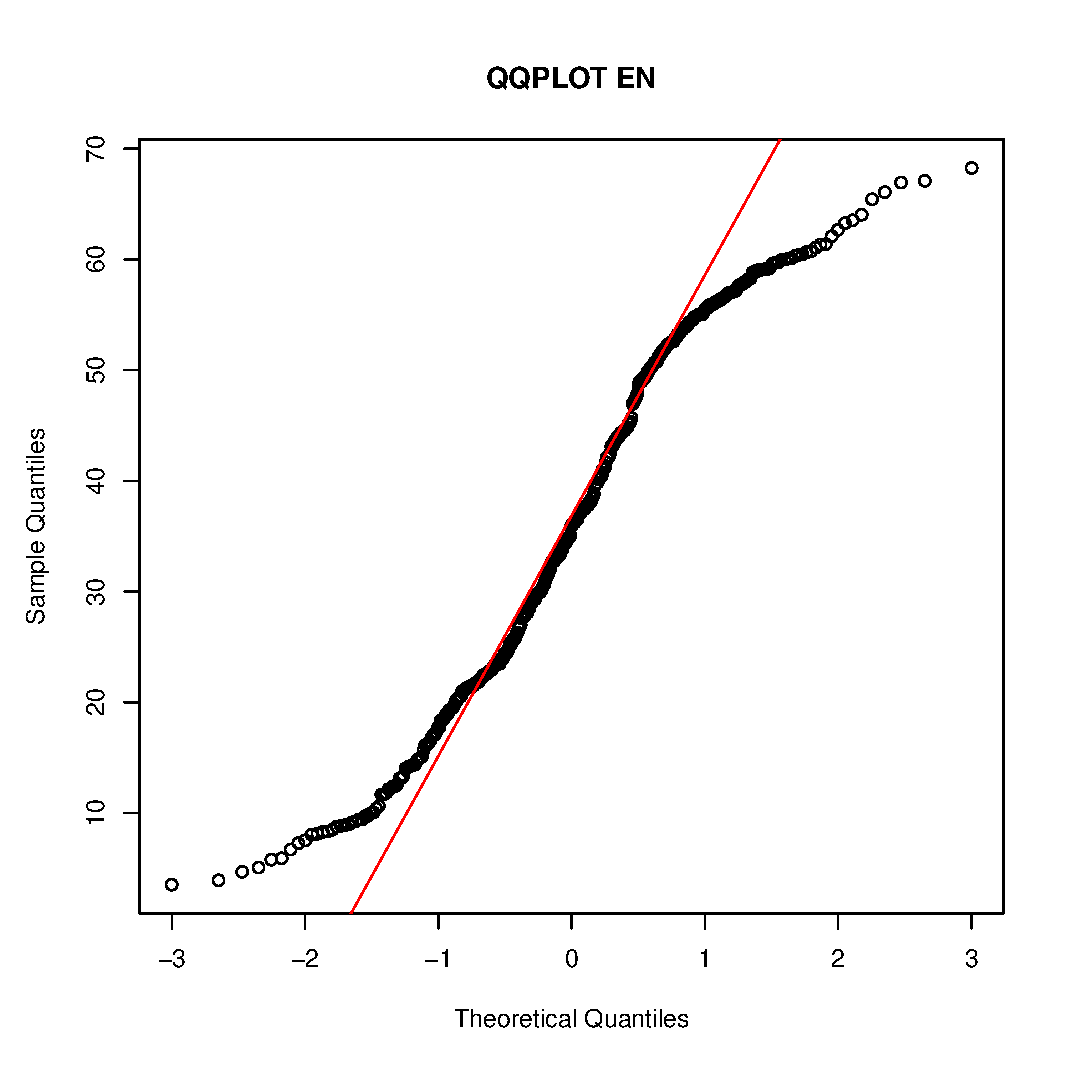
\includegraphics[height=5cm,width=6cm]{figures/EN_QQ.eps}
%	\caption{QQ-plot of EN monthly capacity factor time series ranging from January 1981 to December 2011.}
%	\label{qq_EN}
%\end{figure}

\begin{figure}[htbp]
	\centering
	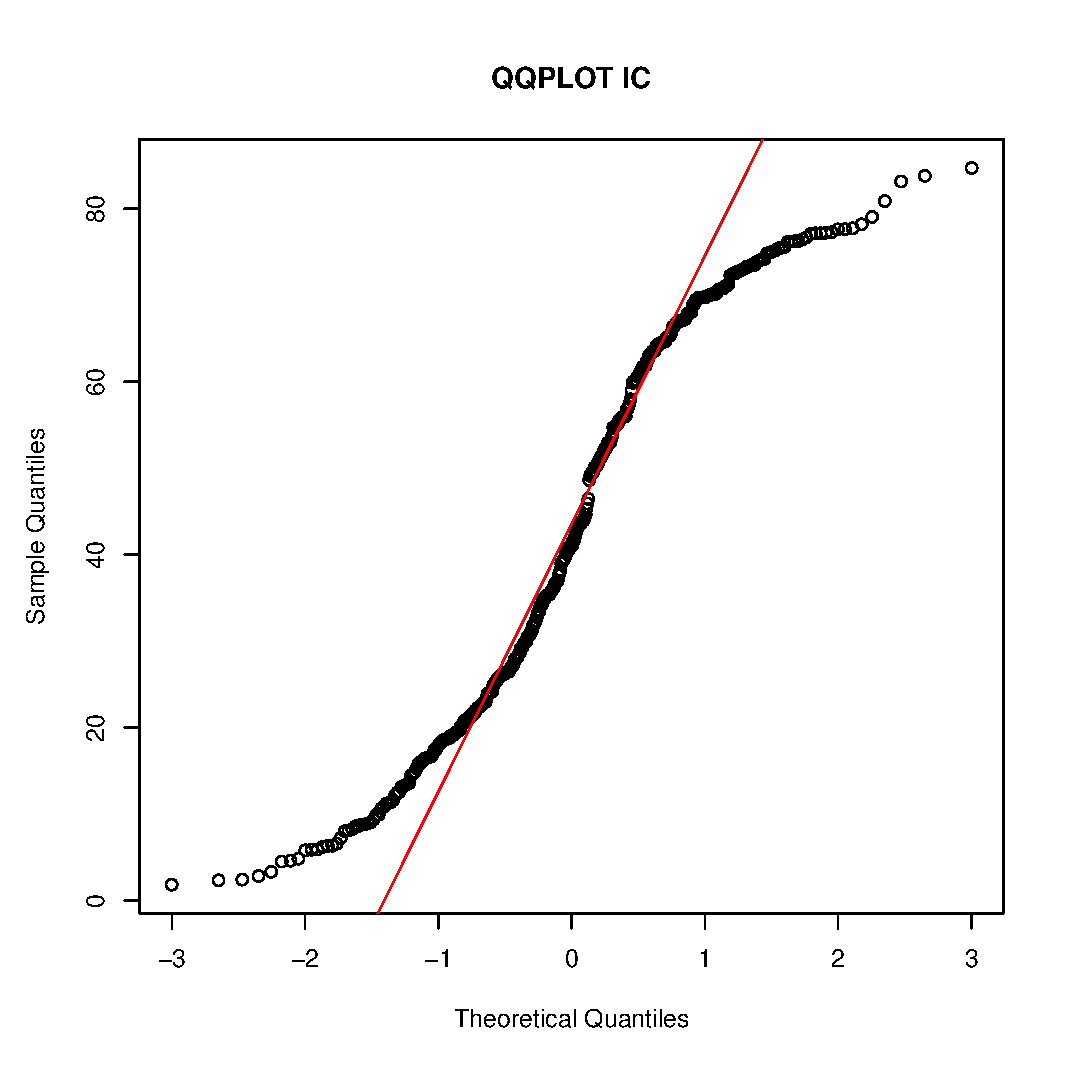
\includegraphics[height=5cm,width=6cm]{figures/IC_QQ.eps}
	\caption{QQ-plot of IC monthly capacity factor time series ranging from January 1981 to December 2011.}
	\label{qq_IC}
\end{figure}

%\begin{figure}[htbp]
	%\centering
	%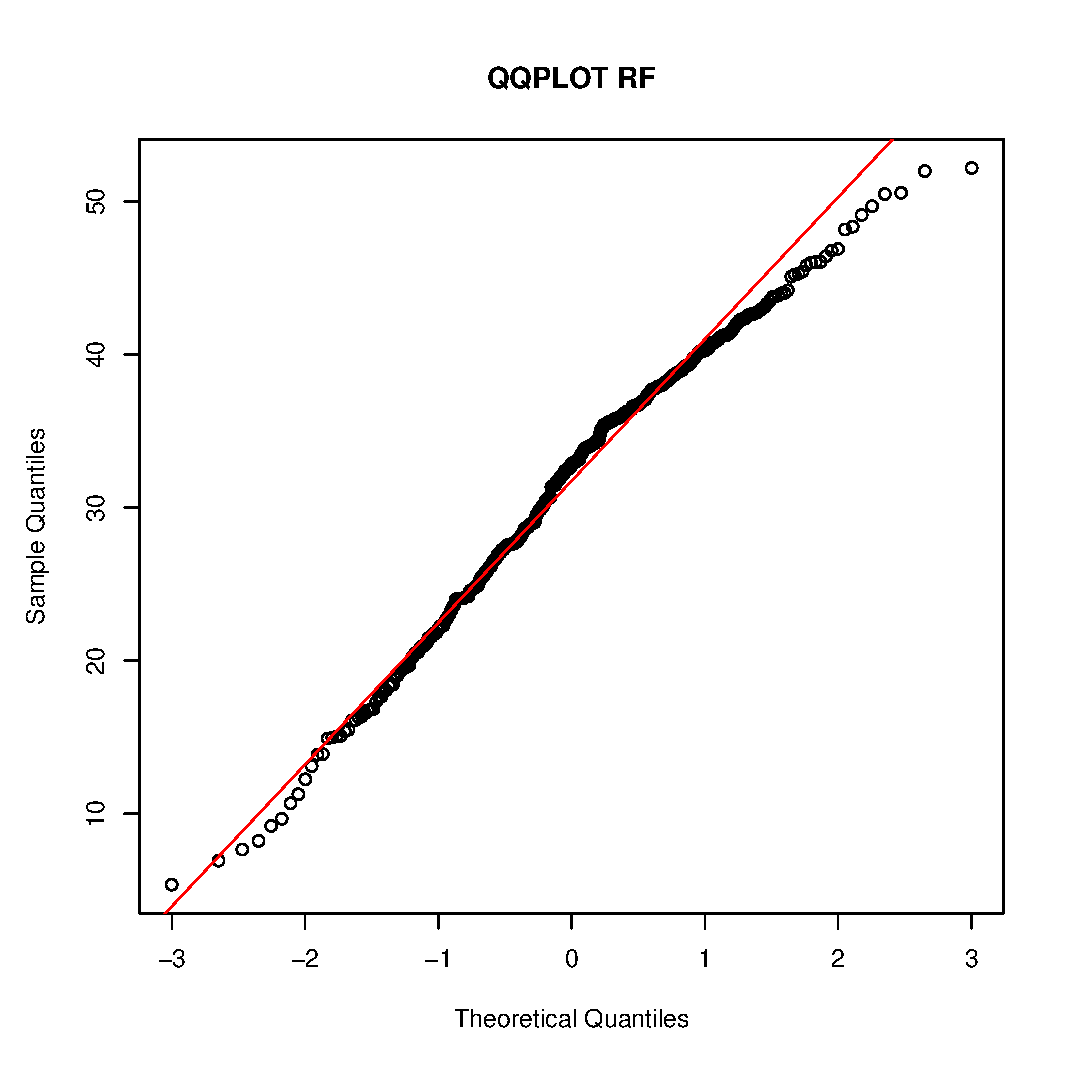
\includegraphics[height=5cm,width=6cm]{figures/RF_QQ.eps}
	%\caption{QQ-plot of RF monthly capacity factor time series ranging from January 1981 to December 2011.}
	%\label{qq_RF}
%\end{figure}

In this study, the same lag structure was used for the three WPG time series, as presented in Equation \eqref{eq:2}. After removing the first and last years of data for initial values estimation and scenario evaluation respectively, maximization of the log-likelihood function resulted in the estimated parameters presented in Table \ref{table1}. Dummy variables $D_t$ were introduced until quantile residuals show no more auto correlation structure. The way to choose in which time index $t$ a dummy variable $D_t$ should be introduced is by checking, after model fit, where $|r_{t,\hat{\theta}_i}|>3$, since under the Gaussianity of the residuals, 3 times the standard deviation reflects an abnormal value. 

\begin{table}[htbp]
\centering
\caption{Maximum likelihood estimation of the beta GAS model applied to three Brazilian wind plants.}
\begin{tabular}{ccccccc}
\multirow{2}{*}{Parameter} & \multicolumn{2}{c}{Rio do Fogo (RF)} & \multicolumn{2}{c}{Icaraizinho (IC)} & \multicolumn{2}{c}{Enacel (EN)} \\
                           & Estim.     & S.E.      & Estim.     & S.E.      & Estim.     & S.E.      \\ \hline
$A_{1}$                    & 0.551      & 0.006     & 0.539     & 0.071      & 0.540      & 0.060     \\
$A_{2}$                    & 0.231      & 0.004     & -0.226      & 0.066     & 0.498     & 0.073     \\
$A_{3}$                    & -0.147     & 0.007     & 0.352      & 0.070     & 0.041      & 0.053     \\
$A_{11}$                   & 0.008      & 0.007     & 0.219      & 0.038     & 0.169      & 0.034     \\
$A_{12}$                   & 0.110       & 0.004     & -0.176      & 0.043     & 0.228     & 0.031     \\
$B_{1}$                    & -0.080      & 0.002     & 1.058      & 0.055     & -0.164      & 0.039     \\
$B_{2}$                    & 0.441      & 0.006     & -0.818     & 0.043     & -0.186     & 0.036     \\
$B_{3}$                    & -0.369     & 0.011     & 0.156    & 0.031     & -0.008       & 0.016     \\
$B_{11}$                   & 0.207      & 0.013     & 0.227      & 0.016     & -0.004       & 0.005      \\
$B_{12}$                   & 0.325      & 0.011     & 0.121      & 0.037     & 0.721      & 0.035     \\
$\omega$                   & 3.139      & 0.019     & 2.571     & 0.260     & 5.485      & 0.780     \\
$\alpha$                   & 9.408      & 0.042     & 10.244     & 0.791     & 9.293      & 0.515     \\
$D_{t=21}^{(Set, 1983)}$   & -          & -         & 2.320      & 0.287     & 1.447          & 0.247         \\
$D_{t=22}^{(Oct, 1983)}$   & -          & -         & 2.021      & 0.309     & 3.610      & 0.481     \\
$D_{t=29}^{(May, 1984)}$   & -          & -         & -0.031      & 0.641     & -          & -     \\
$D_{t=129}^{(Sep, 1992)}$  & -          & -         & 3.349      & 0.317     & 1.675      & 0.386     \\
$D_{t=130}^{(Oct, 1992)}$  & -          & -         & -          & -         & 1.189      & 0.345     \\
$D_{t=165}^{(Sep, 1995)}$  & -          & -         & 1.460      & 0.264     & -          & -     \\
$D_{t=241}^{(Jan, 2002)}$  & -          & -         & -          & -         &-1.527      & 0.582     \\
$D_{t=308}^{(Aug, 2007)}$  & 1.771      & 0.346     & -          & -         & -          & -         \\
$D_{t=309}^{(Sep, 2007)}$  & 2.384      & 0.369     & -          & -         & -          & -         \\
$D_{t=345}^{(Sep, 2010)}$  & 3.004      & 0.277     & -          & -         & -          & -         \\
$D_{t=346}^{(Oct, 2010)}$  & -          & -         & -1.462     & 0.350     & -          & - \\\hline
\end{tabular}
\label{table1}
\end{table}

Finally, to investigate correct model specification, a fully detailed analysis in the quantile residuals was undertaken and reported in Table \ref{table2}. Jarque-Bera test for normality (under the correct specification of the beta density, the residuals should be normally distributed), Ljung-Box test for absence of autocorrelation and Ljung-Box on the squared residuals to check for ARCH effects were considered (both were conducted using until lag 30). As reported in Table \ref{table2}, there were no rejections of the null hypothesis in none of the tests, hence it can be concluded that the proposed beta GAS models are adequate to describe the three time series of WPG.

\begin{table}[htbp]
%\begin{table}[]
\centering
\caption{P-values of standard diagnostic tests.}
\begin{tabular}{c|ccc}
\hline
{\bf Test}      & {\bf Rio do Fogo} & {\bf Icaraizinho} & {\bf Enacel} \\ \hline
Normality       & 0.242             & 0.582            & 0.386         \\
Autocorrelation & 0.174             & 0.854            & 0.127         \\
Arch effect     & 0.703             & 0.479            & 0.175         \\ \hline
\end{tabular}
\label{table2}
\end{table}

%{\color{red} After model fit, one should follow steps \ref{step1_uni}-\ref{step3_uni} of Part I in \ref{univariate_modelling} to generate future scenarios of WPG time series for each one of the $K$ units. We produced 2000, $m=1,...,2000$, scenarios for each of the $h$ steps ahead forecasting horizon $h=1,2,...,12$. The median, at each step $h$, of those scenarios are compared to those obtained from fitting a SARIMA model to the logarithm of the WPG time series, adopting the same dummy variables $D_t$ which were used to fit the beta GAS models. Nevertheless, when using the SARIMA model, to obtain the prediction for the original WPG time series, these values have to be exponentiated. As it is known, exponentiation of Gaussian values can result in unrealistically large values for the original variable. This will not be the case with GAS models since from the outset the chosen probability model is appropriate to the support of the response variable. Goodness of fit results as shown in Table \ref{tablefor} indicates that our model seems competitive when compared to the benchmark SARIMA model.}

Although the forecasts of our beta GAS model are superior to the ones obtained using a simple SARIMA model, we advocate that the main contribution of the proposed framework here is not to improve the conditional mean forecast. Alternatively, the main goal of the proposed methodology is 1) to enhance the whole PDF description for individual time series, e.g., extreme quantiles are better approximated under the proposed framework, and 2) to enhance the multivariate description by capturing the spatial dependence among time series (generally located at different geographical areas) through a time-varying copula.

\begin{table}[htbp]
\centering
\caption{Forecasting evaluation between beta GAS(12,12) and SARIMA model.}
\begin{tabular}{c|cccc}
\hline
Modelo                 & Medidas        & RF    & IC     & EN     \\ \hline
                       & RMSE           & 5.639 & 6.181  & 8.736  \\
beta GAS(12,12)        & MAE            & 5.209 & 5.021  & 7.346  \\
                       & Pseudo R$^{2}$ & 0.834 & 0.941  & 0.875  \\ \hline
                       & RMSE           & 7.566 & 10.668 & 9.737  \\
SARIMA                 & MAE            & 6.263 & 7.675  & 8.222  \\
                       & Pseudo R$^{2}$ & 0.809 & 0.831  & 0.859  \\ \hline
\end{tabular}
\label{tablefor}
\end{table}

In the following we will conduct the multivariate modeling of the three WPG time series using the second step GAS procedure previously described in \ref{step1_multi}-\ref{step4_multi} of Part II in \ref{multivariate_modelling}. The copula parameters were estimated and its values are displayed in Table \ref{tab_3}. Regarding its degrees of freedom, it was estimated using profile likelihood process which resulted in $\hat{\nu}=340$. Such value of degrees of freedom points out that the proposed elliptical copula reduces itself to a time-varying Gaussian copula, which makes perfect sense since we are dealing with monthly data.
   
\begin{table}[htbp]
\centering
\caption{Maximum likelihood estimation of the second step GAS model applied to the PIT variables of three Brazilian wind plants.}
\label{my-label2}
\begin{tabular}{c|cc}
\hline
\multirow{2}{*}{{\bf Parameter}} & \multicolumn{2}{c}{{\bf t-GAS}}                       \\
                                 & \multicolumn{1}{l}{Estim.} & \multicolumn{1}{l}{S.E.} \\\hline
$\Omega$                         & 1.589                      & 0.063                    \\
$\Pi$                            & 0.354                      & 0.017                    \\
$\Upsilon$                       & 0.425                      & 0.083                    \\\hline
\end{tabular}
\label{tab_3}.
\end{table}
   
From Table \ref{tab_3}, it follows that all parameters are statistically significant at 5\%, or less. The value of the parameter $\Pi$ plays a key role here, since it reinforces the fact that dependence structure among these three WPG time series might not be static over the analyzed period. One should note that, if such values are zero or not significant, in the limit, the time varying correlation matrix will be constant, which means that our framework reduces itself to a constant copula model.
   
To introduce spatial dependence information into the joint scenarios of WPG, one should follow the steps provided in Section \ref{dep_scenarios} to simulate scenarios of the \emph{t-GAS} model. To evaluate the quality of the simulated values, we compared the empirical quantiles obtained from the \emph{t-GAS} and SARIMA model 12 steps ahead against the historical monthly quantiles of the original WPG series (both in the original scale) \footnote{The historical monthly quantiles of the original WPG was calculated by first segmenting the WPG time series of wind plant $i \in K$ into 12 monthly time series, i.e., $\{Y_{Jan}^{(i)},..., Y_{Dez}^{(i)}\}$. The same was applied to the simulated sets from \emph{t-GAS} and SARIMA models.}. The quantiles $Q^{(\alpha\%)}\, \forall \,\alpha \in \{0.05, 0.10, 0.5, 0.9, 0.95 \}$ of each set were calculated and plotted in Figures \ref{analise_cenarios_gas} and \ref{analise_cenarios_SARIMA}, where the lines are the monthly quantiles of the simulated set from one of the models, while the geometric figures represent the historic monthly quantiles of the real data set.


\begin{figure}[htbp]
\centering
%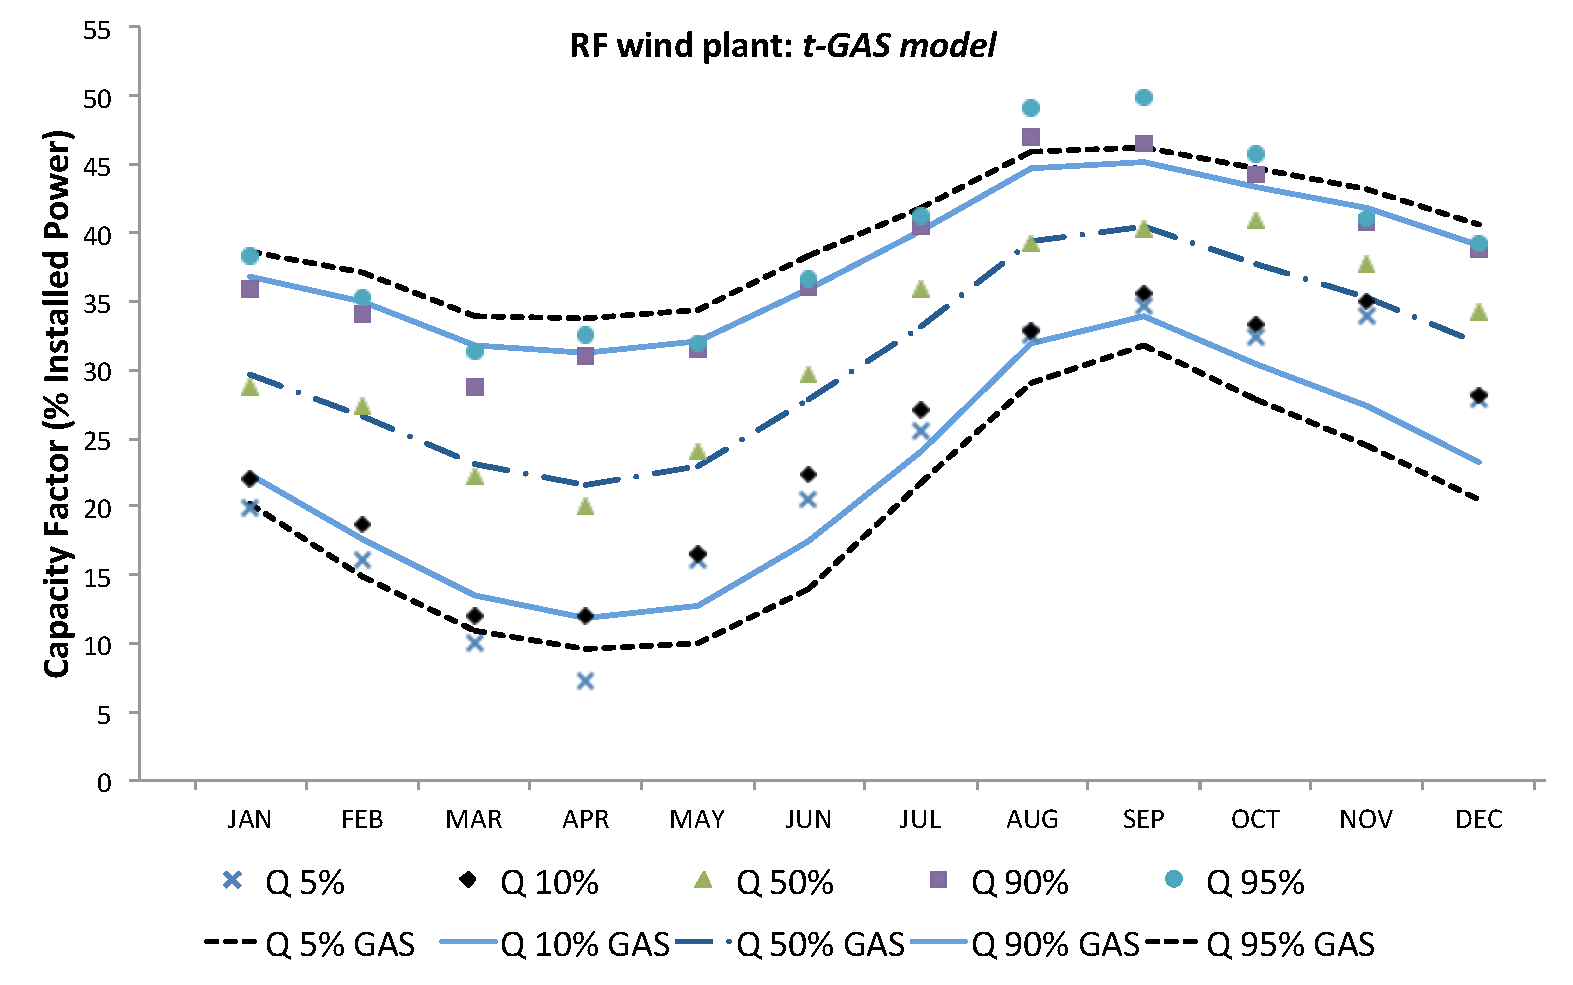
\includegraphics[height=5.5cm,width=9.0cm]{figures/RF_BETA_GAS.pdf}
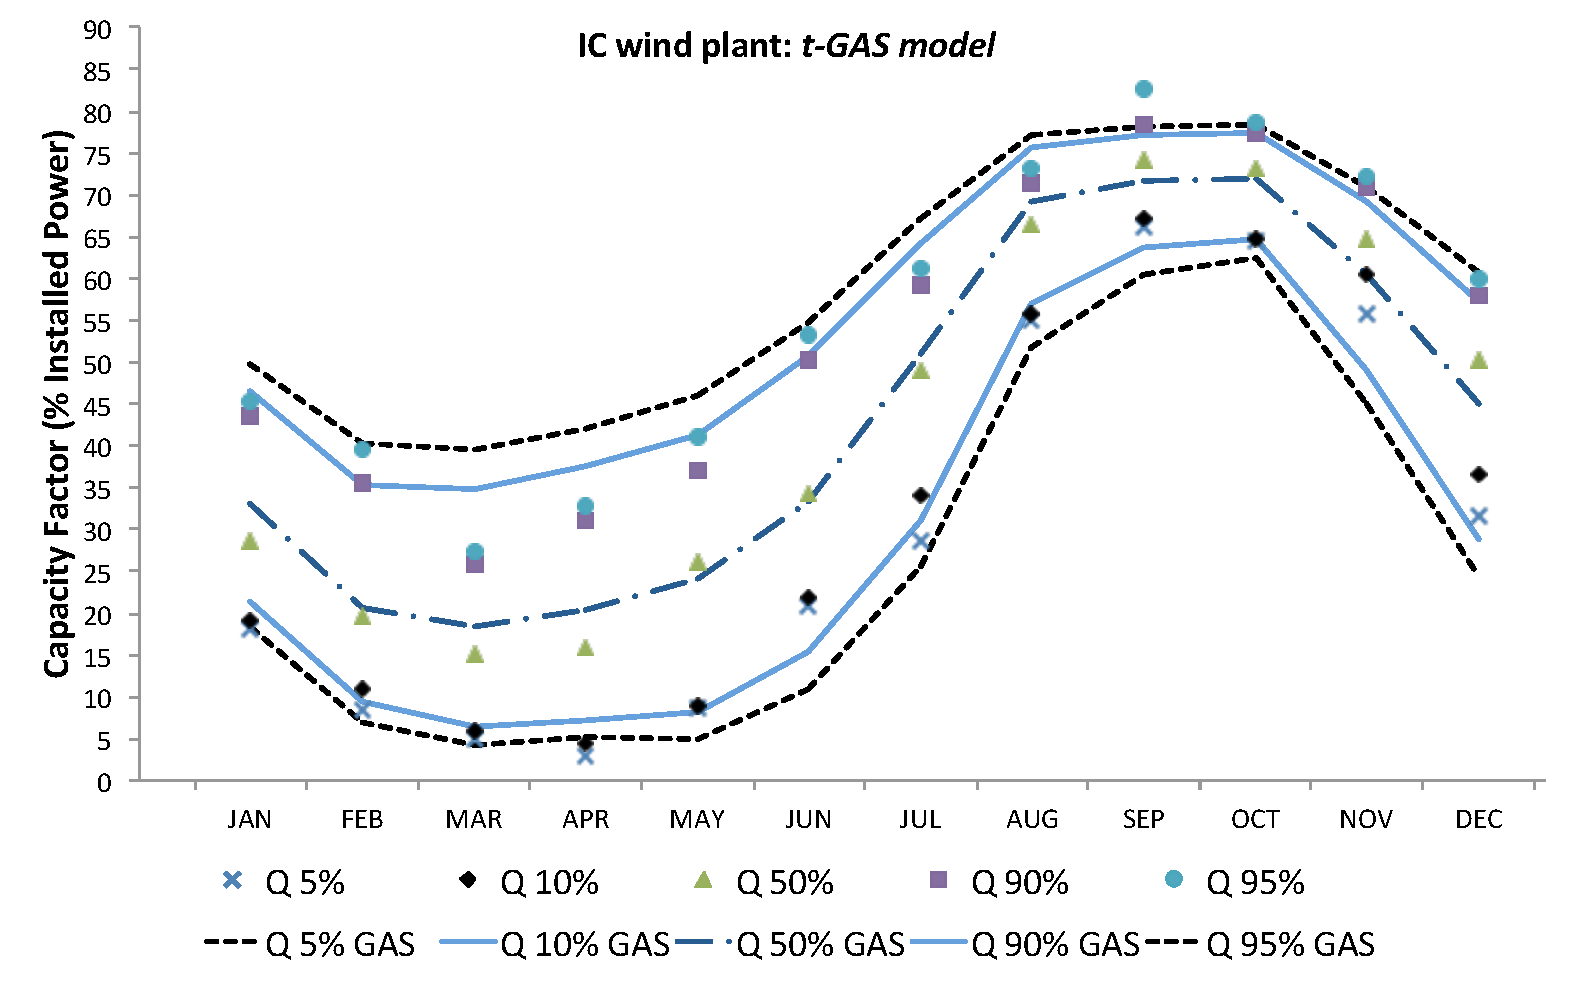
\includegraphics[height=5.5cm,width=9.0cm]{figures/IC_BETA_GAS.pdf}
%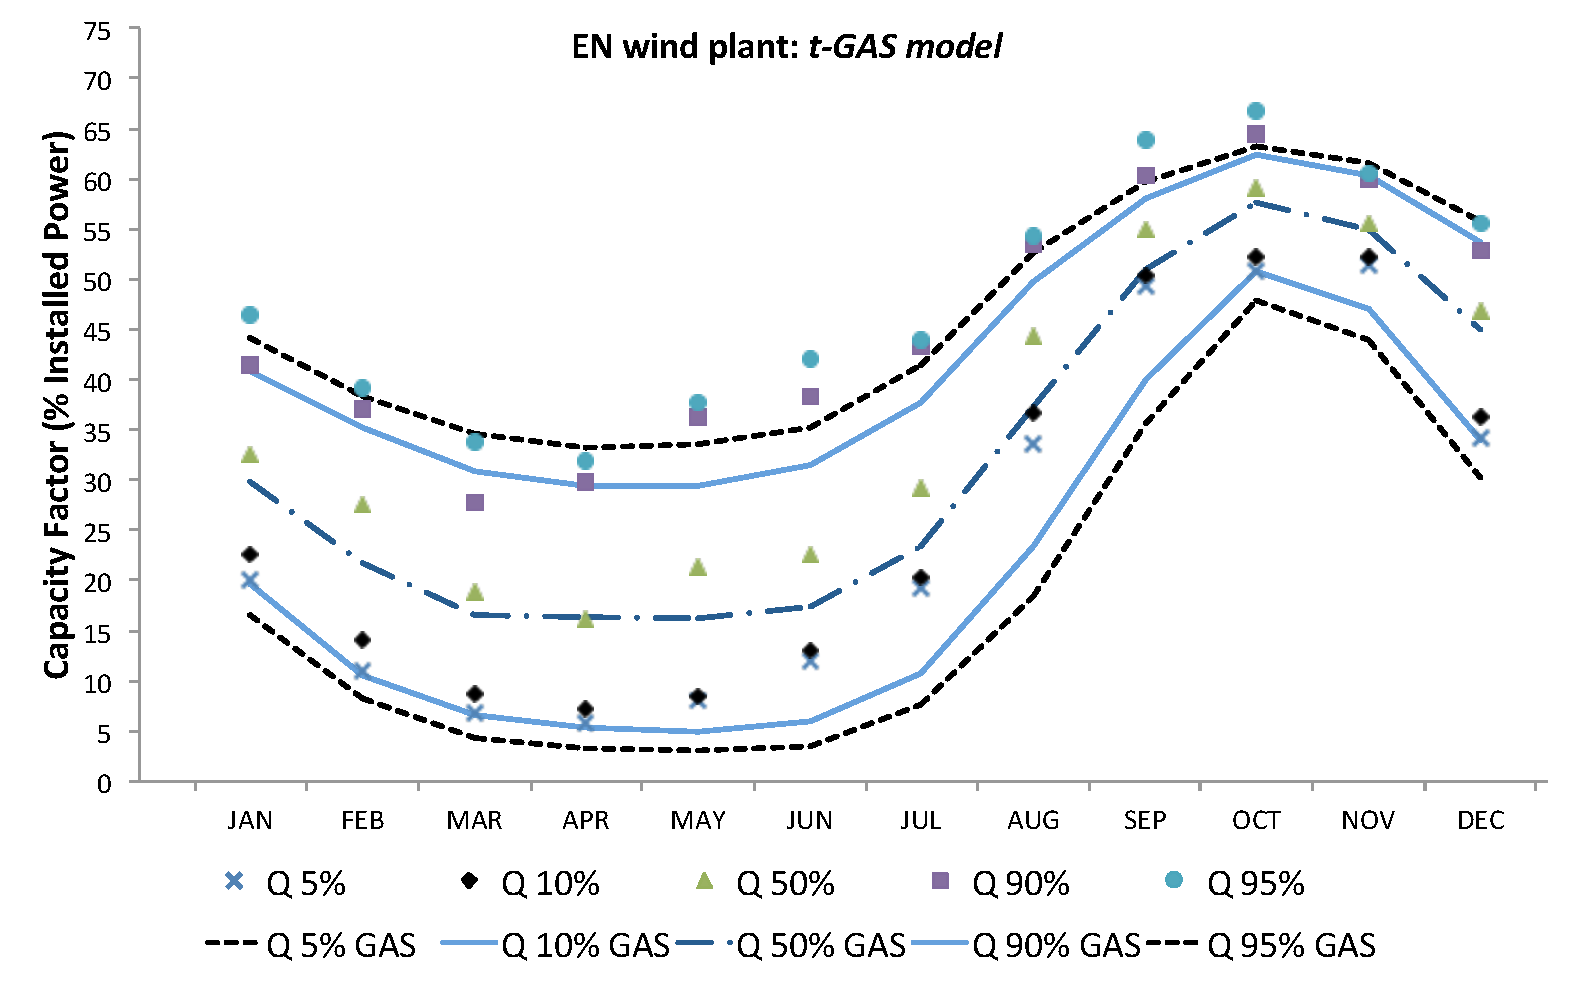
\includegraphics[height=5.5cm,width=9.0cm]{figures/EN_BETA_GAS.pdf}
\caption{Scenario evaluation of the year of 2011 through beta \emph{t-GAS} model against the real data set.}
\label{analise_cenarios_gas}
\end{figure}


\begin{figure}[htbp]
\centering
%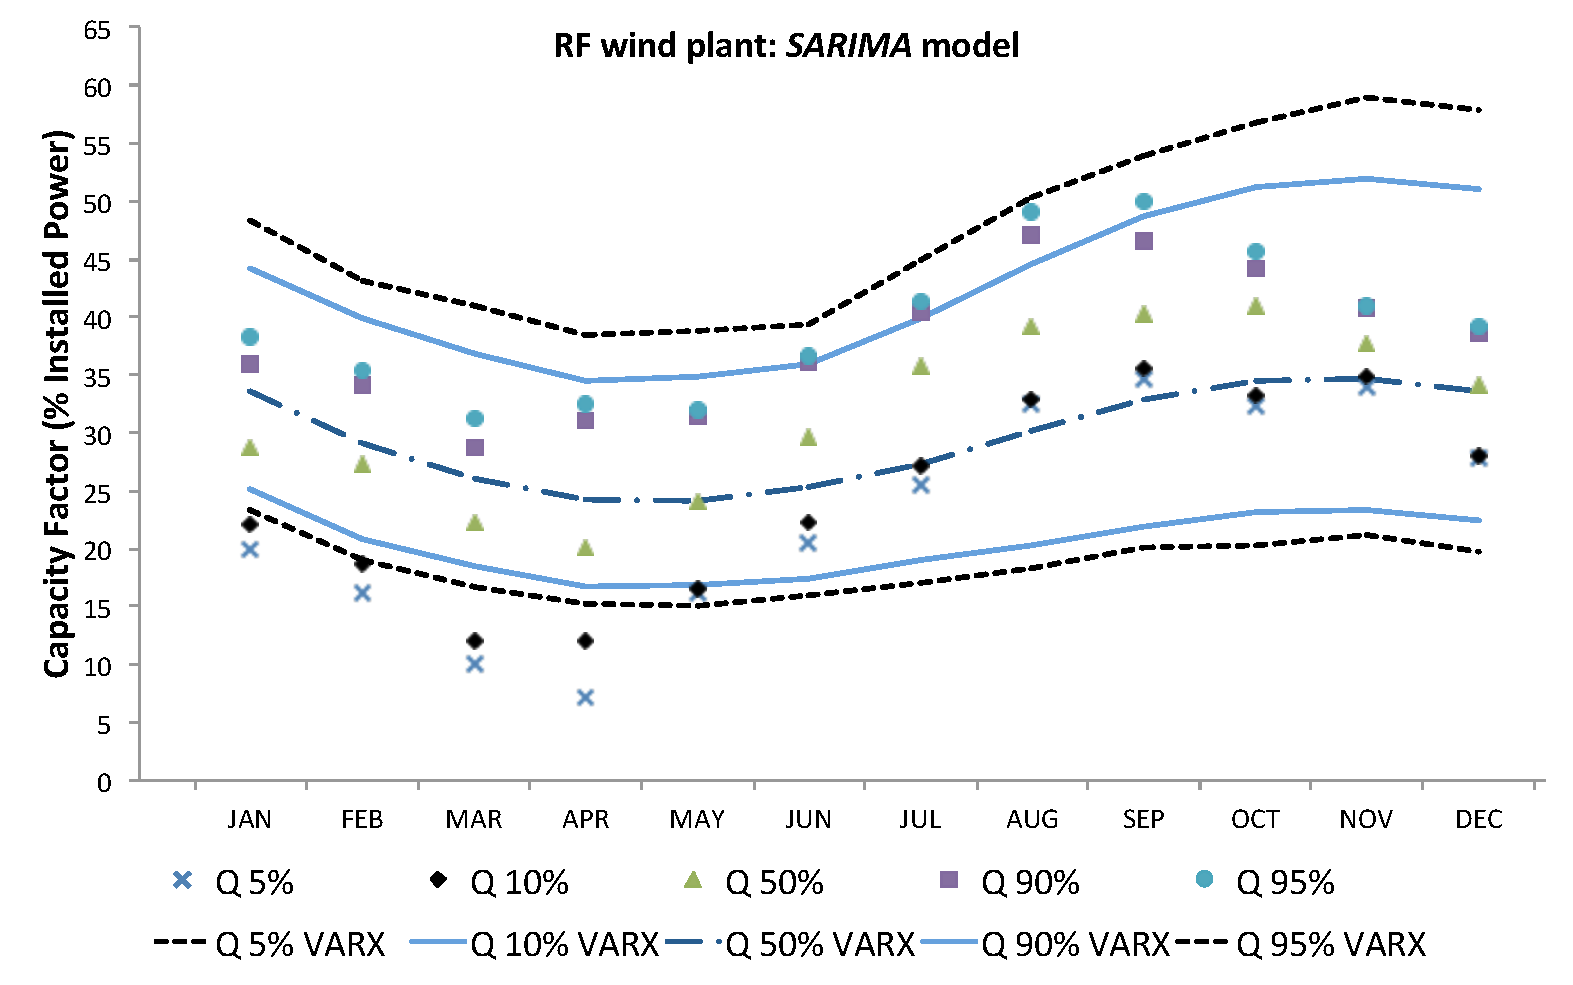
\includegraphics[height=5.5cm,width=9.0cm]{figures/RF_COM_LOG.pdf}
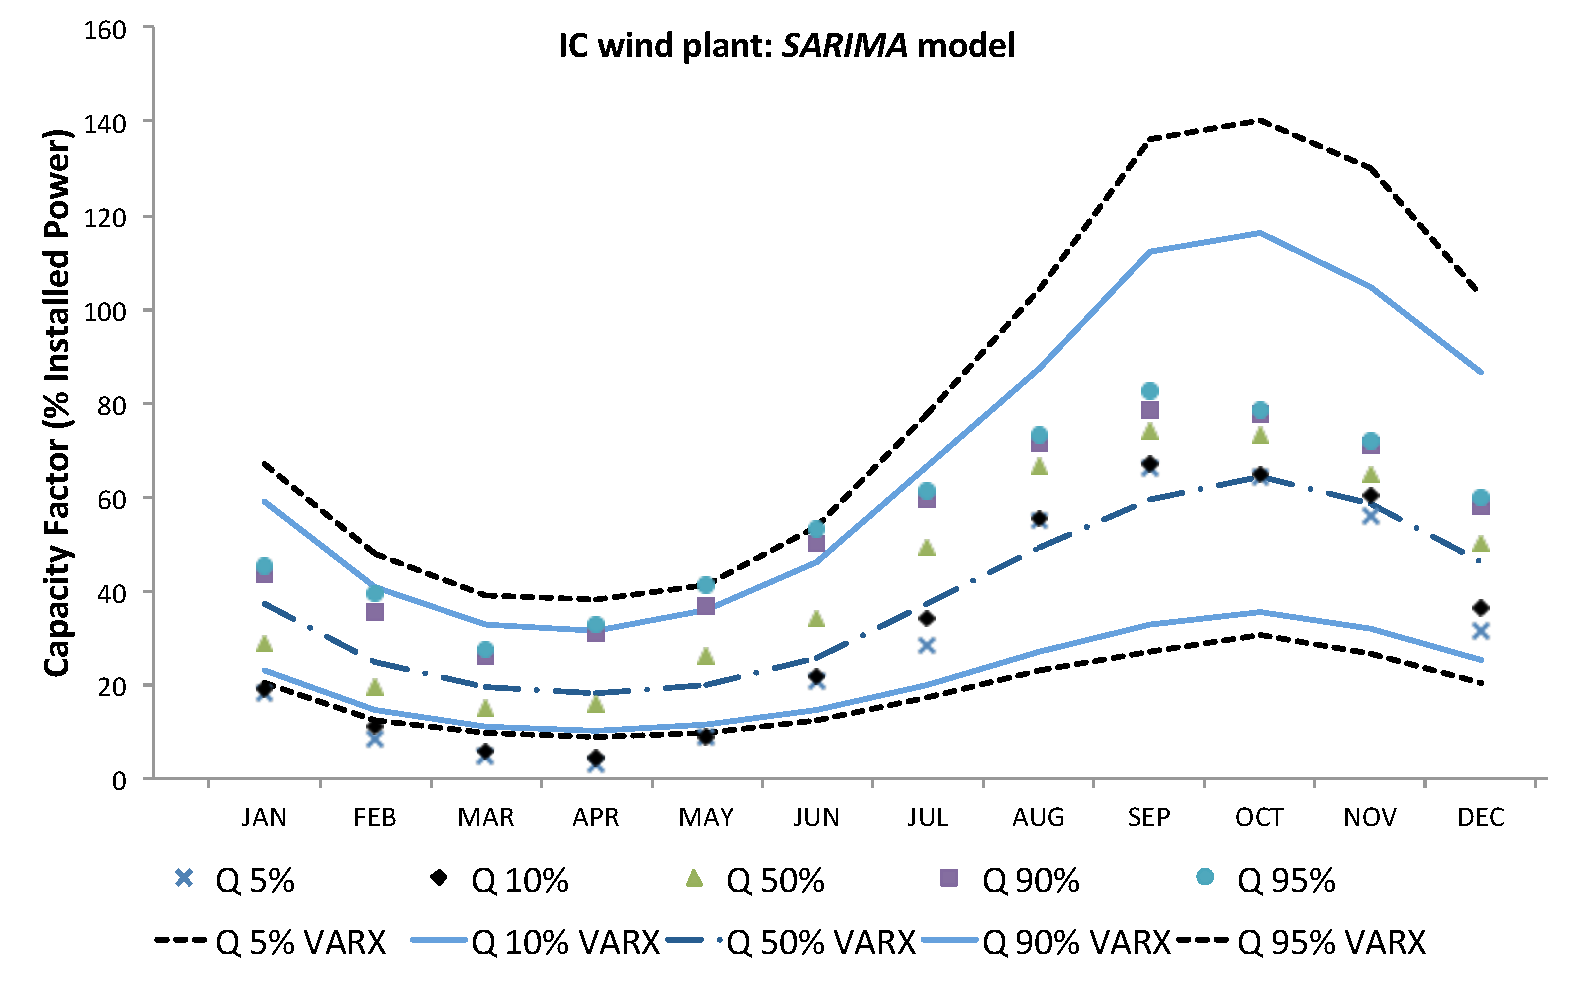
\includegraphics[height=5.5cm,width=9.0cm]{figures/IC_COM_LOG.pdf}
%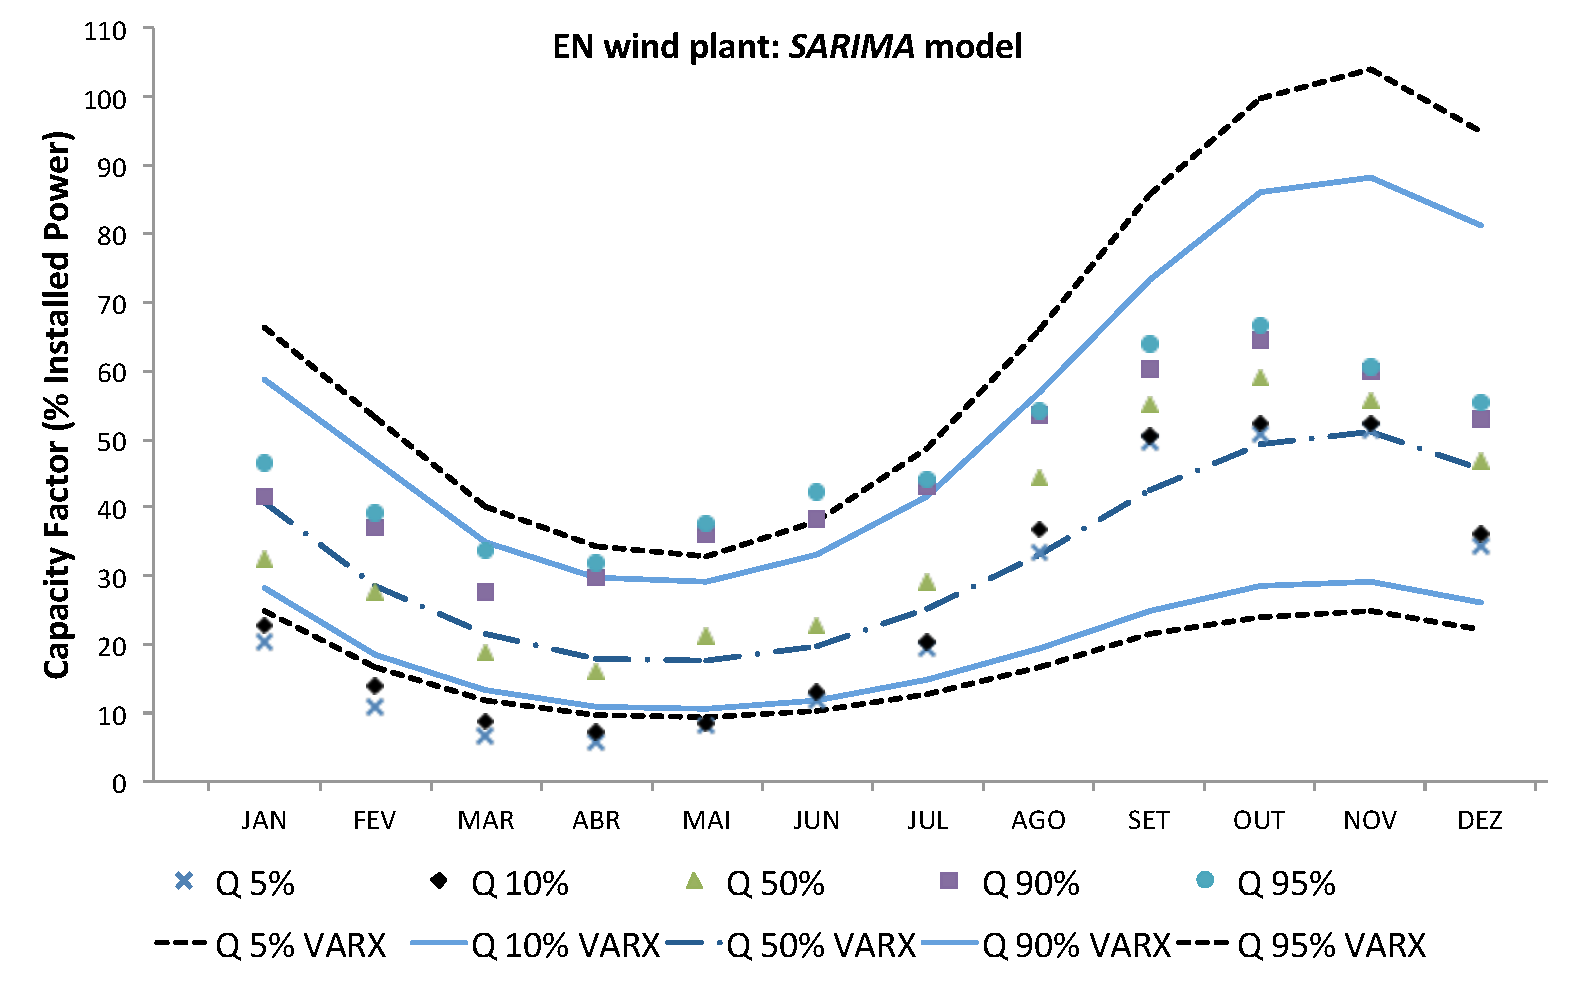
\includegraphics[height=5.5cm,width=9.0cm]{figures/EN_COM_LOG.pdf}
\caption{Scenario evaluation of the year of 2011 through SARIMA model against the real data set.}
\label{analise_cenarios_SARIMA}
\end{figure}

Note that the quantiles from the simulated sets using our \emph{t-GAS} model seems to be more reasonable and likely to the ones estimated from the real data set, while SARIMA ones are far beyond the historical quantiles. This provides evidences on the distortion brought by the anti log transformation, since we fitted a Gaussian SARIMA model to the log of the three WPG time series wind plants (EN,IC,RF).

To reinforce our findings, we calculate the reliability of our quantiles as described in \cite{Wan2017}. Low reliability on the extreme quantiles could prejudice the decision-making process. Based on the definition of quantile, the empirical proportion of quantile $q_t^\alpha$ is defined as,
\begin{align} 
\hat{P}_Q^\alpha = \frac{1}{T}\sum_{t=1}^T \eta_t
\end{align}
\noindent
where T is the total number of observations, and $\eta_t$ denotes the indicator of quantiles $\hat{P}_Q^\alpha$ defined by,
\begin{align} 
\eta_t=
\begin{cases}
1, & y_t \leq q_t^\alpha\\
0, & y_t > q_t^\alpha.\\
\end{cases}
\end{align}

The reability will provide the deviation between the empirical proportion $\hat{P}_Q^\alpha$ and nominal proportion $\alpha$ of the predicted quantiles. The average proportion deviation (APD) is then calculated by $\hat{PD}_Q^\alpha = \hat{P}_Q^\alpha - \alpha$ and provided in Table \ref{APD}. The closest to zero, the higher reability of the estimated quantiles $q_t^\alpha$.

\begin{table}[htbp]
\centering
\caption{Average proportion deviation (APD)}
\label{APD}
\begin{tabular}{@{}l|lll|lll@{}}
& \multicolumn{3}{c}{GAS}                                                  & \multicolumn{3}{c}{SARIMA}                                               \\  \hline
$\alpha$ & \multicolumn{1}{c}{RF} & \multicolumn{1}{c}{EN} & \multicolumn{1}{c}{IC} & \multicolumn{1}{c}{RF} & \multicolumn{1}{c}{EN} & \multicolumn{1}{c}{IC} \\ \hline
5\%   &     3.33\%            &  3.33\%               &   3.33\%                & 11.67\%                &  11.67\%               &  11.67\% \\
10\%  &     -1.67\%            &  6.67\%               &   6.67\%               & 15.00\%                &  15.00\%               &  6.67\%  \\
50\%  &     3.33\%            &  8.33\%               &  8.33\%                 & 16.67\%                 &  16.67\%                &  25.00\%  \\
90\%  &     1.67\%            &   1.67\%               &  -6.67\%               & 10.00\%                 &  10.00\%               &  10.00\% \\
95\%  &     -3.33\%           &  -3.33\%               &  -3.33\%               & 5.00\%                 &  5.00\%                &  5.00\%  \\ \hline
\end{tabular}
\end{table}
%{\color{red} @PARADO AQUI: IR DIRETO PARA A DEFINICAO DE Q e falar do mecanismo de atualizacao}.
By the results of Table \ref{APD} it is possible to argue that the scenarios generated by our proposed framework, specially on extreme quantiles, are very well estimated which is an expected outcome due to the fact that the copula model acts on the tail behaviour of the predictive density. In addition, we also implemented the conditional coverage Value at Risk exceedances test of Christoffersen \cite{christoffersen1998evaluating} to check the coverage level of each predictive density against real data in Table \ref{cristofersen}. Non significant p-values reinforce the idea that the proposed model is adequate to fit the WPG time series. 
\begin{table}[htbp]
%\begin{table}[]
\centering
\caption{P-values conditional coverage Value at Risk exceedances test of Cristoffersen considering a coverage level of 95\%.}
\begin{tabular}{c|ccc}
\hline
{\bf Coverage level}      & {\bf RF} & {\bf IC} & {\bf EN} \\ \hline
\emph{t-GAS} model   & 0.305             & 0.305           & 0.305        \\
SARIMA               & 0.035             & 0.035           & 0.035   \\ \hline     
\end{tabular}
\label{cristofersen}
\end{table}

As expected, p-values of Cristoffersen test applied to SARIMA predictive densities are all significant, considering a coverage level of 95\%. In contrast, predictive densities produced by \emph{t-GAS} model are all non-significant, using the same level of coverage.

% ===== Sec. V - Conclusion ===== %

\section{Conclusion}\label{Conclusion}

In this paper we proposed a framework to simulate joint scenarios of WPG time series taking into account the spatial dependence among different units. Such scenarios are deeply demanded for the development of medium- and long-term studies for power-system planning under uncertainty of renewable energy generation. Our methodology seems fruitful and have several benefits when comparing against a benchmark SARIMA model, regarding its parametric features and the straightforward way to estimate and generate extreme quantiles. The proposed framework was derived making use of a recently proposed class of time-series models with time-varying parameters and arbitrary non Gaussian distribution, known as Generalized Auto Regressive Score models (GAS). When adopting such models, one does not need to transform WPG and work with the $log$ of the observed data point. Our framework is taylor made for the range of values that WPG time series can assume. In addition, copula models were used to input spatial dependence into the generated joint scenarios. Its use is unarguably better when comparing the extreme scenarios to the ones generated by the SARIMA model.
\section*{Acknowledgment}

Henrique Hoeltgebaum, Cristiano Fernandes and Alexandre Street acknowledge support from CNPq/Brazil.

%\IEEEtriggeratref{17}
\bibliographystyle{IEEEtran}
\bibliography{Bibhenriquinho}

%\begin{IEEEbiographynophoto}{Henrique Hoeltgebaum} has a B.Sc. degree in Statistics from Federal University of Rio Grande do Sul, Brazil and a M.Sc. degree in Electrical Engineering from PUC-Rio, Brazil. Currently he is pursuing a Ph.D degree in Electrical Engineering at the same university.
%\end{IEEEbiographynophoto}

%\begin{IEEEbiographynophoto}{Cristiano Fernandes} has a M.Sc. degree in Electrical Engineering from PUC-Rio, Brazil and a D.Sc. in Statistics from London School of Economics.
%\end{IEEEbiographynophoto}

%\begin{IEEEbiographynophoto}{Alexandre Street} (S'06, M'10) holds the degrees of M.Sc. and D.Sc. in Electrical Engineering (Operations Research) from PUC-Rio, Brazil. 
%\end{IEEEbiographynophoto}

\appendices

\section{Gas mechanism for the multivariate Student t distribution}\label{FirstAppendix}

In this appendix we present the elements of the GAS mechanism $s_t$, $\nabla_{t}$ and $\mathcal{I}_{t|t-1}^{-1}$ for the multivariate Student t distribution, but first let us define a few matrix notations. The matrix $\mathcal{D}_{K}$ is a duplication matrix given by $\mathcal{D}_{K}vech(C) = vec(C)$ and the Kronecker product of two matrixes $C$ and $D$ is denoted by $C \otimes D$. In case $C=D$, $C_{\otimes}$. By convenience the operator $vec(C)$ creates a column vector from a matrix $C$ by stacking the column vectors of $C$ while $vech(C)$ also creates a column vector stacking only column vectors of the inferior triangular part of $C$. For a full detailed review on linear algebra operators, please see \cite{abadir2005matrix}.

Now, the proposed GAS mechanism in\cite{creal2011dynamic} to update the time varying correlation matrix $\Sigma_t$ using a multivariate Student t is given by 
  
\begin{align} 
\nabla_{t} = \frac{\partial \ln p(\tilde{y}_{t}|\Sigma_{t};\nu)}{\partial f_{t}} =& \frac{1}{2} \Psi_{t}^{'} \mathcal{D}_{K}^{'}\Sigma_{t\otimes}^{-1}[w_{t}\tilde{y}_{t\otimes}-vec(\Sigma_{t})] \label{nabla} \\
\mathcal{I}_{t|t-1} = E[\nabla_{t}\nabla_{t}^{'}] =& \frac{1}{4} \Psi_{t}^{'} \mathcal{D}_{K}^{'}J_{t\otimes}^{'}[gZ-vec(I)vec(I)^{'}] \label{info} \\ & J_{t\otimes}\mathcal{D}_{K}\Psi_{t} \nonumber
\end{align}
\noindent
where $\Psi_{t}=\partial vech(\Sigma_{t})/\partial f_{t}^{'}$ which will be presented next in Equation \eqref{derivPSI}, the scalar $w_{t}=(\nu+K)/(\nu-2+\tilde{y}_{t}^{'}\Sigma_{t}^{-1}\tilde{y}_{t})$ reduces the effects of outliers, once the former quantity is divided by $\tilde{y}_{t}^{'}\Sigma_{t}^{-1}\tilde{y}_{t}$. Matrix $J_{t}$ is defined as $\Sigma^{-1}_{t}=J^{'}_{t}J_{t}$, which can be obtained by any matrix decomposition procedure. In our application in Section \ref{Application}, we adopted Cholesky decomposition. The scalar $g=(\nu+K)/(\nu+2+K)$ and the elements of the square matrix $Z$ of dimension $K\times K$, are given by
\begin{align} 
Z[(i-1)\cdot k+\ell,(j-1)\cdot k+m]=\delta_{ij}\delta_{\ell m} + \delta_{i\ell}\delta_{j m} +  \delta_{im}\delta_{j \ell}
\end{align}
\noindent
with $i,j,\ell,m=1,...,K$, assuming $\delta_{ij}$ equals to 1 if $i=j$ and zero otherwise. 

As previously discussed, the key to define a copula framework in \cite{creal2011dynamic} is to use the following specification of $\Psi_{t}$ in Equations \eqref{nabla}-\eqref{info},
\begin{equation} \label{derivPSI}
\Psi_{t} = \mathcal{B}_{K}D_{t\otimes}\Delta^{-1}_{t\otimes}[\mathcal{D}_{K}-(\Delta_{t} \oplus Q_{t})\Delta_{t\otimes}^{-1}W_{\Delta_{t}}\mathcal{S}_{\Delta}]\mathcal{S}_{Q}
\end{equation}
\noindent
where $\mathcal{S}_{Q}=I$ since $f_{t}=vech(Q_{t})$. The matrix $W_{\Delta_{t}}$ is initially calculated using a diagonal matrix of dimension $K^{2} \times K^{2}$ with elements of the main diagonal equals to $0.5vec(\Delta^{-1}_{t})$, and later the columns of zeros are eliminated. The matrix $\mathcal{S}_{\Delta}$ is a selection matrix, with ones and zeros, given by $diag(\Delta^{2}_{t})=\mathcal{S}_{\Delta}vech(Q_{t})$. The operator $\oplus$ is given by $C\oplus D=(C\otimes D)+(D\otimes C)$. In addition, $\mathcal{B}_{K}=(\mathcal{D}_{K}^{'}\mathcal{D}_{K})^{-1}\mathcal{D}_{K}^{'}$ is a duplication matrix composed by only zeros and ones, with more lines than columns. $\Delta_{t}$ is a diagonal matrix which elements are the square root of the elements contained in the main diagonal of $Q_{t}$

\end{document}
